%%
%%  chapter00.tex - Obstacle Detection and Planning for Autonomous Vehicles based on Computer Vision Techniques
%%
%%  Copyright 2014 Néstor Morales <nestor@isaatc.ull.es>
%%
%%  This work is licensed under a Creative Commons Attribution 4.0 International License.
%%

\graphicspath{{./images/chapter00/bmps/}{./images/chapter00/vects/}{./images/chapter00/}}

\addchap{Introduction}\label{ch:chapter00}


They should not allow humans to drive. We are fuzzy, disrespectful with rules and easily distracted. Maybe this is the reason for which driving has been considered one of the top ten causes of death by the \ac{WHO}\footnote{\href{http://www.who.int/features/factfiles/roadsafety/en/}{http://www.who.int}}. According to it, every year there are 1.24 million road traffic deaths worldwide, most of them vulnerable road users (pedestrians, cyclists, motorbikes...). Of these, a lot of them could have been avoided if rules were followed, such as speed limits, alcohol/drugs consumption, passive safety systems, etc. 

Fortunately, since 2007 at least 88 countries have reduced the number of road traffic deaths. This improvement of the road safety is probably due to a better awareness of the drivers about the dangers of not following the traffic rules and the existence of better roads. But probably, the rise of the use of \ac{ADAS} in commercial vehicles is helping the drivers to avoid dangerous situations, usually motivated by a distraction.

Driving is difficult, too. There are many rules, with hundreds of pages to memorize \citep{schwarzenegger2007california}, many exceptions and a lot of unpredicted situations. Moreover, it is time consuming. On average, a US citizen expends 38 hours a year stuck in traffic \footnote{\href{http://www.theatlantic.com/business/archive/2013/02/the-american-commuter-spends-38-hours-a-year-stuck-in-traffic/272905}{http://www.theatlantic.com}}. That is a lot of time, that could be used for more interesting and productive things.

\begin{figure}
  \centering
  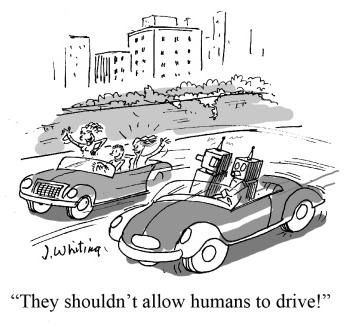
\includegraphics{CarCartoon}
%   \caption{Credits: Jim Whiting.}
% \label{fig:cp00_humans_not_drive}
% Fuente:
% http://webserver.computoredge.com/online.mvc?zone=SD&issue=2945&article=cover&session=
\end{figure}

For all these reasons, and many more, the amount of research related to autonomous vehicles has increased a lot in the last years. This kind of research, which was initially restricted to the academic environment, has been adopted by some of the big car manufacturers, like Mercedes-Benz, General Motors, Nissan, Toyota, Audi, etc. The existence of driverless vehicles is getting closer to be a reality. In fact, many states of the United States have already approved laws that take into account this possibility, being the first of them the state of Nevada in 2011. Also, countries like the United Kingdom have approved similar laws.

Apart from the aforementioned benefits, an increase in the use of autonomous cars would allow many more:
\begin{itemize}
 \item As said, higher safety due a to a decrease in the number of traffic accidents.
 \item Reduced traffic congestion, as the roads can increase their capacity.
 \item Vehicle occupants can spend their time in things other than driving.
 \item Higher speed limits.
 \item Occupants are not tied to constraints like being under age, blind, intoxicated, etc.
 \item Alleviation of parking scarcity and reduction of space required for vehicle parking.
 \item Reduction in the need for traffic police and vehicle insurance.
 \item Physical road signs will not be needed anymore: autonomous cars could receive necessary communication electronically.
 \item Smoother ride.
\end{itemize}

In order to make this a reality, vehicles must fulfill a set of requirements. They should be able to follow the driving rules that allow a safe coexistence with the human drivers, as well as being adaptable for a wide range of situations. Above all, they should detect the obstacles in the road and avoid them in safe conditions. 

% Many works have also been done about this last topic. In this thesis, we want to contribute to this research area. With this objective in mind, we propose a set of algorithms and methods which will contribute to a safe trip, oriented to the case of the autonomous vehicles and, in particular, to the prototype Verdino, which will be introduced later. Theses methods will be described, and their advantages and drawbacks analyzed. Also, we will propose some improvements for the algorithms presented.

\section{Problem Statement}\label{ch:chapter00_01}

% The usage of computer vision for environment understanding applications related to autonomous robotic platforms has been widely studied over the years, leading to the creation of some prototype vehicles \citep{Maurer1996,Pomerleau1996,Broggi1999} which demonstrated that negotiating moderately complex and dynamic situations in real time was possible, albeit challenging. However, it was only with the development effort driven by the DARPA Challenges \citep{Buehler2007, Buehler2009} that the technology required to provide reliable operation both in off-road and urban scenarios proved to be within reach.

The methods described in this thesis are intended to be used in our testing platform, an autonomous robotic prototype called Verdino. This platform, which is explained in more detail in section \ref{ch:chapter00_03}, consists on an electric vehicle used for the transportation of people in closed areas (such as golf courses, urbanizations, etc.). This has been modified to make it able to drive autonomously, operated by a computer which is installed on board. For this purpose, the original steering, brakes and accelerator have been modified, and many sensors have been mounted on it, including many cameras. The final goal of this prototype is being able to transport people in pedestrian areas, without the need of a driver.

In this thesis, we propose different methods which will be used, in the first place, for the detection of obstacles in the environment of a vehicle. In the first part of this document, we describe a set of methods thought for this purpose, each of these making use of a different technique. This allows comparing the advantages and disadvantages of each of them, from the point of view of the proposed application. Once the prototype is finished, it will not work in a controlled environment in which everything is static. Instead of that, the areas in which Verdino will travel are usually crowded, with many pedestrians which are usually in a relaxed mood, so we can not trust they will simply move their selves out of the way of the vehicle. Because of that, we need to be able to detect the presence of obstacles and situate them in a map, so they can be avoided. Furthermore, as the obstacles will be usually moving, it would be desirable to know where they are going to, so we allow the vehicle taking more intelligent decisions. Based on this, we can define the requirements for the obstacle detection method as:

\begin{itemize}
 \item Getting a reasonable obstacle detection rate using as input the images provided by the cameras onboard. That means that the method should be able to work with images obtained from non static cameras.
 \item Ability to localize the obstacles in the map.
 \item The method should be able to work in real time conditions.
 \item The method should be also able to detect the obstacles independently of the weather or environment conditions.
 \item We should be able to track the obstacles along frames.
\end{itemize}

The methods proposed in this thesis represent several attempts to solve the problems listed above. Initially, we just solved some of them separately. In the two final approaches described, we are able to fulfill all the requirements proposed simultaneously, but through different approaches in each case. The advantages and disadvantages of each are discussed at the end of this document.

Once obstacles are detected, we need to avoid them. In the second part of the thesis, we describe the method used by the prototype to travel around the map. This method comprises two tasks: the first one computes a trajectory that starts in the position of the vehicle and ends in the target to which we want to move. If we had a \ac{RNDF}, we would not need to compute this trajectory, but as Verdino travels in an unstructured environment, this step is needed. In the second step, Verdino does the calculations needed to follow the computed trajectory. In this step, we want the vehicle to be able to follow the track but, at the same time, we also want to have enough flexibility in the commands generated to ensure that it is able to abandon the track if necessary in case we want to avoid an obstacle.

% The vehicles that successfully took part to this series of events had to integrate planning and actuation capabilities with a sensing suite capable of coping with harsh environments, heavy traffic and wide temperature ranges, while keeping functional over extended amounts of time. Most competitors relied on high-end active sensors \citep{Urmson2008, Montemerlo2008, Bacha2008, Kammel2008}, with some notable exceptions \citep{Broggi2006, Broggi2010}.

Going back to the methods tested for the detection and tracking of obstacles, we have implemented up to four different approaches. In the next paragraphs, we will introduce them. These are very heterogeneous and the methods in which they are based have few in common. Due to that, they must be introduced separately.

The first approach we explored is inspired in the work by \cite{primdahl2005change},  \cite{diego2011video} or \cite{vallespi2012prior}. This is based on the fact that, in an image, a high percentage of the scene represented usually corresponds to static objects. Based on that, it looks quite straightforward to think that, having an image representing the same area without obstacles, it is possible to detect the obstacles in an scene by just comparing it with an image being taken in real time. For that, we obtained a dataset with geo-referenced images from a closed urbanization taken at different times of the day. A description of this database, as well as of the algorithm pipeline used for the comparison between images pairs can be found at chapter \ref{ch:chapter01}.

However, such approach suffers from several drawbacks. First, as we just use one image per frame, we are no able to know the exact position of the obstacle in the real world. Also, the quality of detection is highly tied to the size of the image database, so in big areas we need a huge dataset, with the related space and throughput problems associated to that. If we consider changes due to weather or light conditions, the size of the dataset becomes unmanageable. Finally, we don't know the direction where an obstacle is going to. These are challenging problems that have been solved using different approaches, described in the following chapters.

To solve that, we implemented a new approach in which we isolated the tracking problem with the use of static monocular cameras. Instead of registering pairs of images, we segment the image with the use of foreground extraction techniques, distinguishing between background and foreground. Using the silhouette of the objects in the foreground (which are mainly non-rigid objects, like pedestrians or animals), we apply a non-rigid point set registration algorithm in order to track the different parts of the contour of the obstacles separately. This method can be also used for the completion of the global map of the vehicle, or even for tasks more related to \ac{HMI}. This approach is extensively described in chapter \ref{ch:chapter02}.

However, this method still makes use of a very rudimentary method for the localization of the obstacles (See section \ref{ch:chapter02_01_03}), and it is limited to static cameras. For the application proposed, we need the cameras installed on the top of the moving prototype, so we can not use foreground segmentation methods anymore for the detection of the objects in the road. A simple solution for that is stop using monocular vision, and start using stereo vision. For that purpose, a high number of advanced algorithms has become viable for autonomous driving applications. The problem is that performing a quantitative and meaningful comparison of their performance level, however, is not an easy task, mainly because of the difficulty of producing ground truth information. Existing datasets are small, and either synthetic or taken in controlled environments \citep{Scharstein2002}, thus effectively limiting their usefulness as indicators of the actual algorithms ability to cope with outdoor scenarios. Due to that, it is needed to compare the performance level of some state-of-the-art stereovision-based 3D mapping algorithms in automotive scenarios. This evaluation methodology and the associated results are shown in chapters \ref{ch:chapter03} and \ref{ch:chapter08}.

Apart from the full-dense 3D reconstruction methods, we also explore the possibility of using a simpler (and faster) reconstruction based on stixels, like that described by \cite{badino2009stixel}. In particular, we decided to use the implementation by \cite{benenson2012pedestrian}, due to its fast response (about 100 frames per second). For that, we propose both a two-level and an obstacle level approach, each with its own advantages / disadvantages respect to the other. The method, described in chapter \ref{ch:chapter04}, compares the stixels obtained between frames and tracks the obstacles along the time. This is a good solution for the proposed problem: we can use moving cameras, we can locate the obstacles in the map and we are also able to know the path followed by them. However, the method is highly dependent on the assumptions taken (described in chapter \ref{ch:chapter04}), specially in those related to the ground detection process.

Another approach, which makes use of the dense stereo reconstruction algorithms, as those for which we did the evaluation described above, is mainly inspired in the work by \cite{danescu2012particle}, but also takes some ideas from the work described in \cite{broggi2013}. In this approach, we simplify the 3d reconstructed point cloud into a grid of voxels, each of these representing a certain volume in the world. For each voxel above a given occupancy probability threshold, a set of particles belonging to a particle filter is assigned. Each particle will have a double function: the first, denoting hypotheses (as in the classical particle filter methods); the second, to be used as criteria for the segmentation of the world into different obstacles. In this way, we consider that two contiguous voxels belong to different obstacles if their obtained direction and sense diverges. A more detailed explanation of the method is found in chapter \ref{ch:chapter05}.

At this point, we have an acceptable reconstruction of the surroundings of the vehicle, which includes the localization and tracking of the obstacles in the neighborhood of the cart. But the reconstruction of the environment is not the only challenge that an autonomous vehicle has to deal with. Once that a vehicle has an idea of where it is, and where it wants to go, it also needs to know the best way to reach a certain goal and, more important, how to avoid the harmful elements it has previously detected using the methods described. This allows a safe trip, both for the pedestrians, cars, etc. in the road, and for the vehicle itself.
As said, Verdino is intended to travel in pedestrian areas where most of the obstacles are pedestrians, so its behavior must be mainly reactive in order to give priority to the safety of paths against the efficiency of the route. Also, there is not a clear traveling path, like a road. Instead of that, the vehicle will be moving around an unstructured area, so there is not something like a \ac{RNDF} that allows a fast calculation of the paths that the car will use in order to reach a certain point. Because of that, we must consider two different planning levels:
\begin{itemize}
 \item \textbf{Global Planning:}
 As it is not possible to determine a global trajectory based on a \ac{RNDF}, we must use a method able to deal with changing environments for the calculation of a fast and safe path. The idea is that, having a map of the static obstacles in the environment and with the vehicle properly localized on it \citep{Perea2013mcl}, it will generate a path that will allow reaching this destination as fast as possible. This task, which can be solved easily in static environments using graphs or other similar optimization methods, becomes a little bit more challenging in environments like, for example, a parking lot, in which cars are parking and driving off continuously.
 In chapter \ref{ch:chapter06}, the way in which we solved this problem is described. It is based on the border between classes, which is obtained after training a \ac{MSVM} (See Appendix \ref{ch:appendixSVM} for more information), considering each single obstacle as a separate class. Instead of using this border for classification purposes, as it is usual, we take advantage of the fact that it will be the safest distance to the obstacles, and that this border is smooth. Taking this into account, it makes sense to apply this separation line as our path. Also, the use of a different class for each obstacle allows ensuring that the path is safe enough, even in complicate scenarios, like in pedestrian areas.
 
 \item \textbf{Local Planning:}
 In a lower level, we also need a way to make the vehicle know how to follow the generated path. This problem requires a system able to, several times per second, calculate the best steering angle and speed in order to follow the global plan while avoiding the surrounding obstacles. The method, which is inspired in the work of \cite{chu2012local}, receives as input the current position of the vehicle in the map, its orientation, speed and the steering angle. Also, we provide it with the global plan obtained in the upper level. Finally, a map of the dynamic obstacles in the surrounds of the cart is computed and passed to the algorithm.
 
  This dynamic map can be filled with the information provided by sensors like \acp{LIDAR}, among others. But it can be also computed with the information extracted from cameras, and this is where the works described in the first and second part of this thesis are connected. Detected obstacles are included in the map, so the vehicle is able to avoid them using the calculated steering angle and speed.
 
 The way in which both this map and the speed/steering angle commands is obtained is described in chapter \ref{ch:chapter07}.
\end{itemize}
 
 The whole pipeline of the application developed for this thesis is shown at figure \ref{fig:cp00_pipeline}. 
 

From the images captured in real-time, obstacles are located and passed to the module in charge of the generation of the dynamic costmap. At the same time, the static map is used for the generation of a feasible trajectory. Using the current position and vehicle status, the local planner tries to compute the proper commands in order to follow the global plan while trying to avoid the obstacles included in the dynamic costmap.

\section{Previous Work}\label{ch:chapter00_02}

Research on autonomous vehicles is a topic being studied for a long time. A proof of that is the extensive literature existing about that, in special since the first of the DARPA Challenges \citep{Buehler2007, Buehler2009}. Since then, the literature related to this problem has increased a lot. Moreover, the interest on the use of computer vision in autonomous vehicles is growing, due to the possibilities that images offer to this task if compared to other sensors.

\begin{figure}[h!]
  \centering
  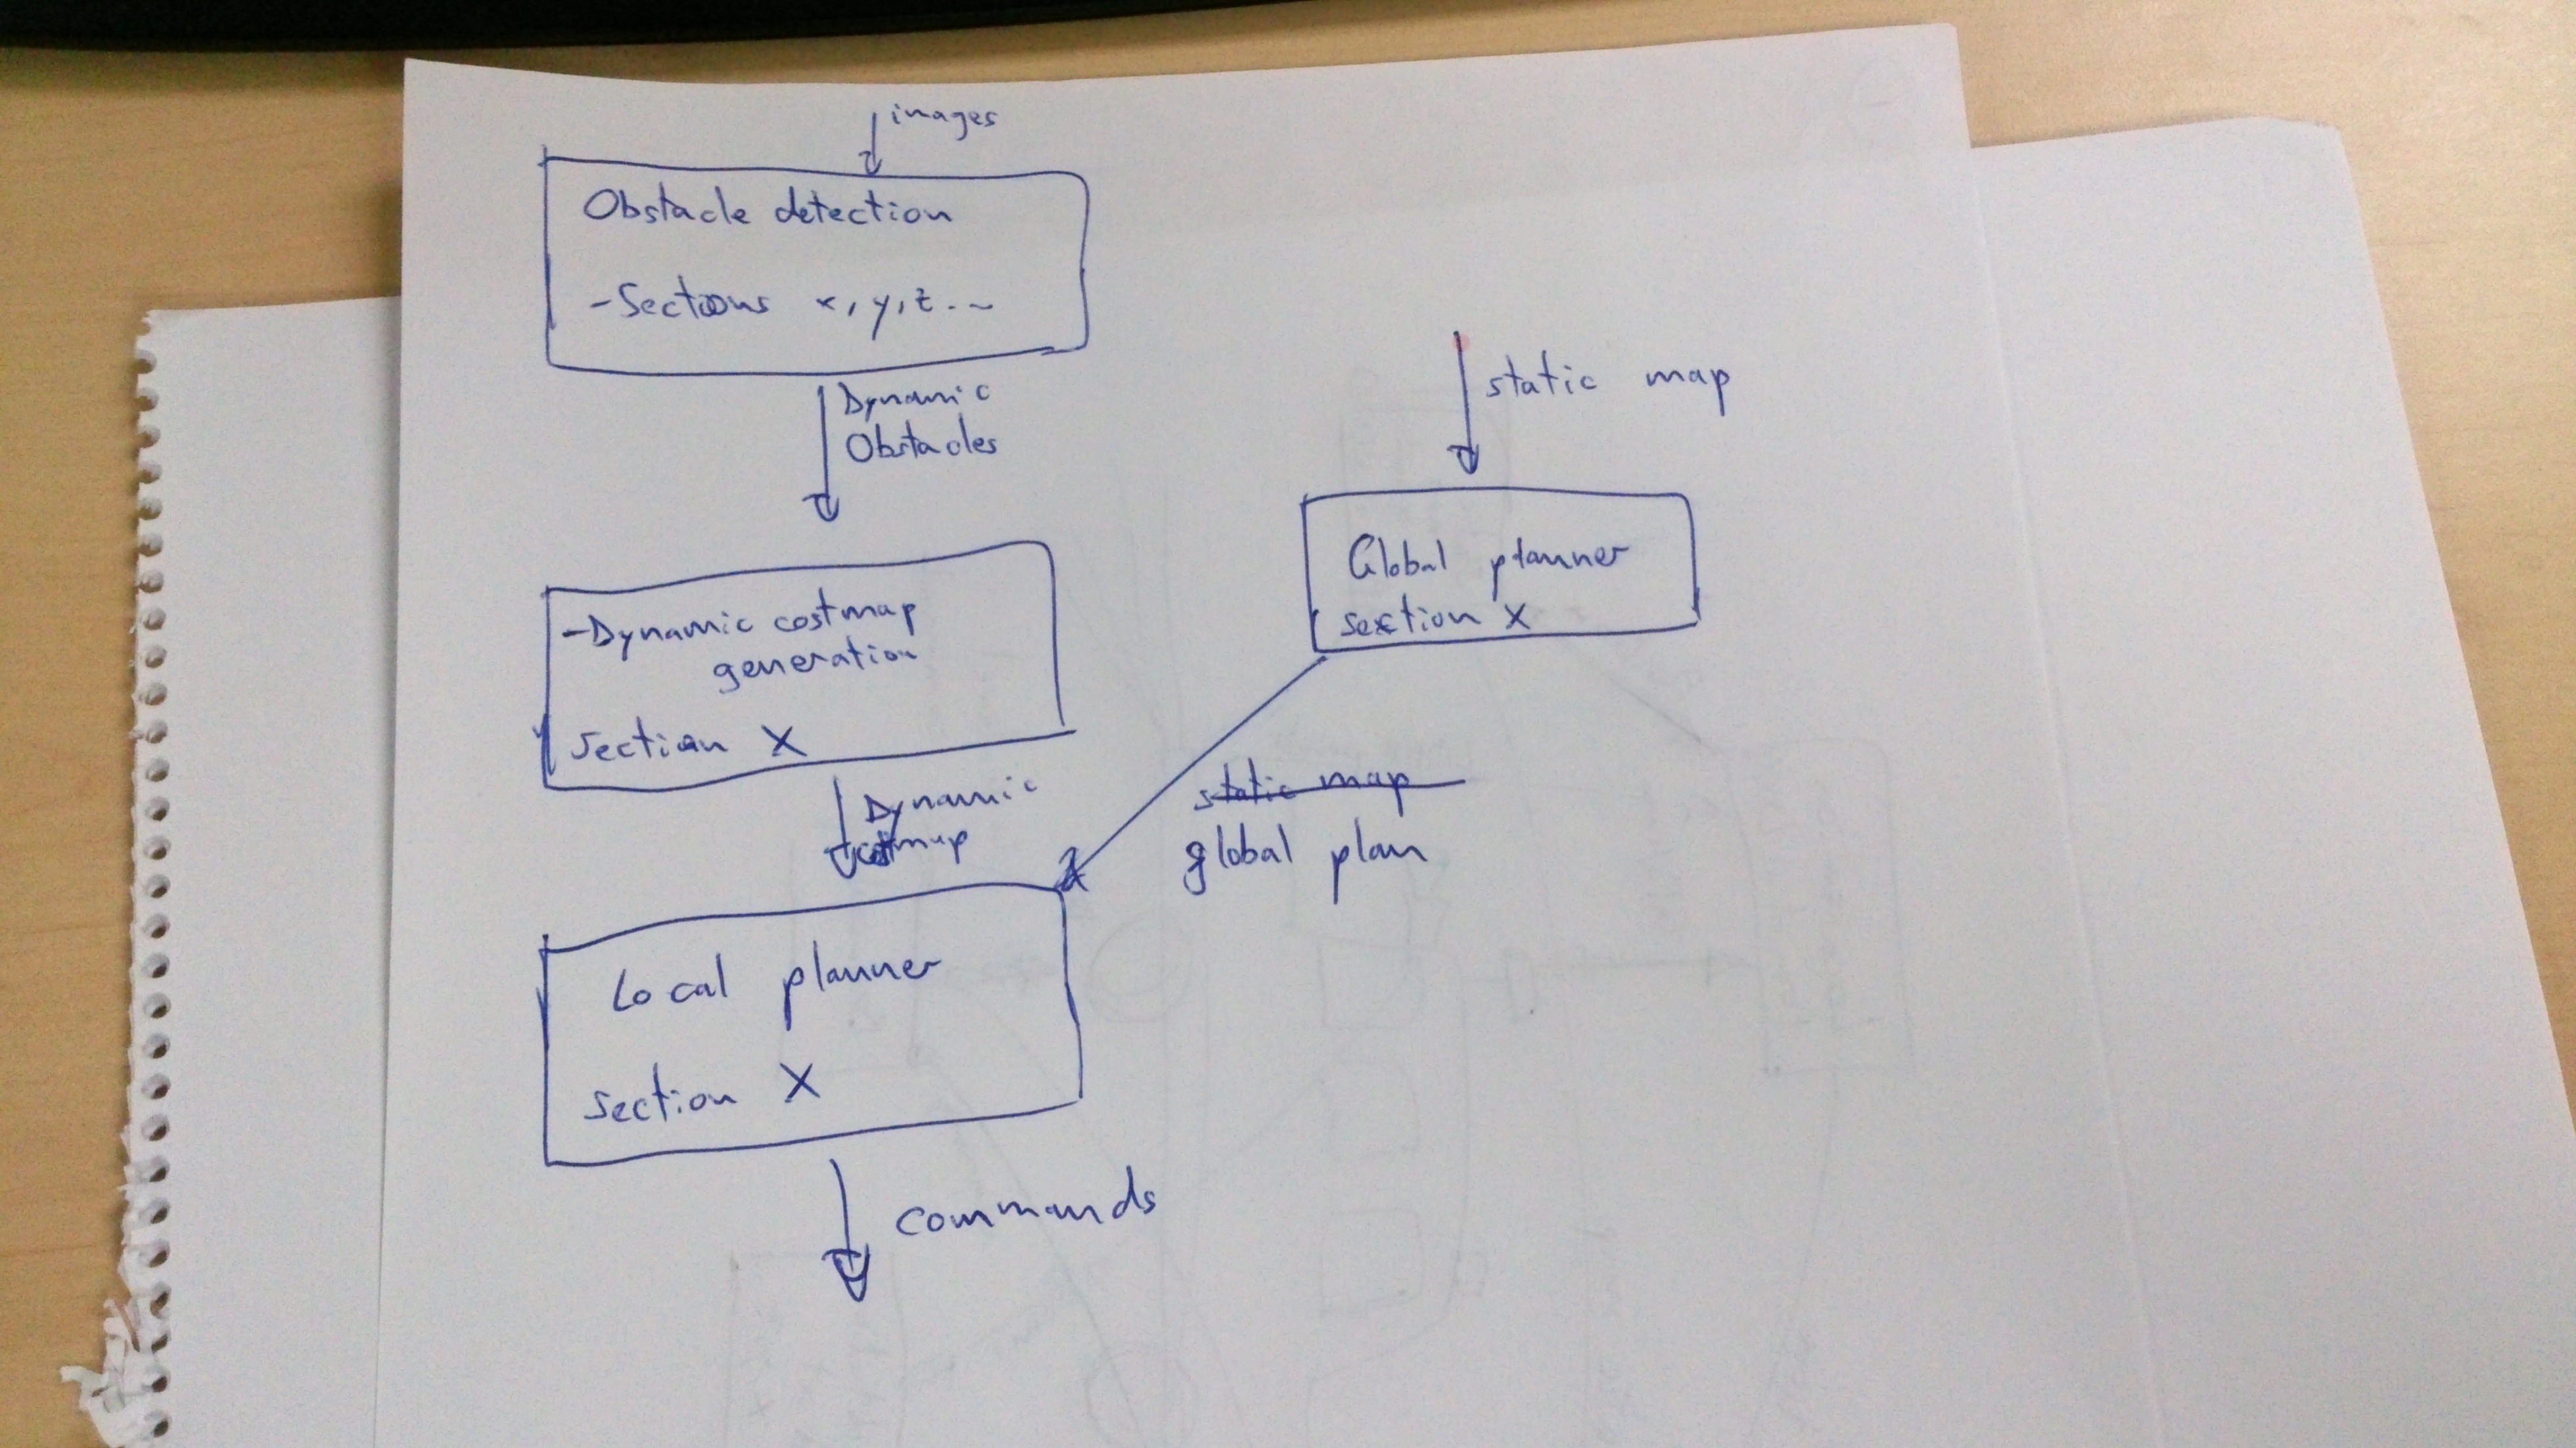
\includegraphics[width=\textwidth,height=\textwidth]{pipeline}
  \caption{Pipeline of the modules described in this thesis.}\label{fig:cp00_pipeline}
\end{figure}

A fast review of the history of autonomous vehicles is listed next:
\begin{itemize}
\item From 1987 to 1995, the EC EUREKA Prometheus Project conducted research on autonomous vehicles. Among its culmination points were the twin robot vehicles VITA-2 and VaMP, driving long distances in heavy traffic.
\item In 1996, the ARGO project modified a Lancia Thema to follow the lane marks in an unmodified highway \citep{Broggi1999}. The culmination of the project was a journey of 1,900\,km over six days on the motorways of northern Italy, with an average speed of 90 km/h. The car operated in fully automatic mode for the 94\% of its journey, with the longest automatic stretch being 55\,km. The vehicle had only two grayscale low-cost video cameras on board and used stereoscopic vision algorithms to understand its environment. 
 \item In 2004, DARPA's Grand Challenge was held in the Mojave Desert region of the United States, along a 240\,km route. This competition consisted on an autonomous vehicles race that must reach to the goal without human intervention and using just a listing of check points between the start and the finish line. None of the robot vehicles finished the route.
 \item In 2005, a second competition was held \citep{Buehler2007}. This time, five vehicles successfully completed the course:
 \begin{itemize}
  \item \emph{Stanley} \citep{thrun2006stanley}, from Standford University.
  \item \emph{Sandstorm} and \emph{H1ghlander} \citep{urmson2004high}, from the Carnegie Mellon University.
  \item \emph{Kat-5} \citep{trepagnier2006kat}, from the Gray Insurance Company.
  \item \emph{TerraMax} \citep{ozguner2004team}, from the Oshkosh Truck Corporation.
 \end{itemize}
 \item In 2007, the third driverless car competition of the DARPA Grand Challenge \citep{Buehler2009}, more known as the DARPA Urban Challenge, was held in Victorville, California. This time, six teams successfully finished the entire course:
 \begin{itemize}
  \item \emph{Boss} \citep{Urmson2008}, from the Carnegie Mellon University.
  \item \emph{Junior} \citep{montemerlo2008junior}, from Standford University.
  \item \emph{Odin} \citep{Bacha2008}, from Virginia Tech.
  \item \emph{Talos} \citep{leonard2007team}, from the Massachusetts Institute of Technology.
  \item \emph{Little Ben} \citep{bohren2008little}, from University of Pennsylvania.
  \item \emph{Skynet} \citep{miller2008team}, from Cornell University.
 \end{itemize}
 \item In 2010, 2012 and 2013, the Korean Autonomous Vehicle Competition (AVC) took place.
 \item In 2010, inside the VIAC Challenge, four autonomous vehicles drove from Italy to China on a 100-day 15,900\,km trip with only limited human intervention (in traffic jams and when passing toll stations). At the time, this was the longest-ever journey conducted by an unmanned vehicle \citep{Broggi2010VIAC}.
 \item In 2011, under the Oxford University's WildCat Project, a Bowler Wildcat based prototype is capable of autonomous operation using a flexible and diverse sensor suite.
 \item In 2011, the Freie Universität Berlin, Led by the AutoNOMOS group, developed two autonomous cars - \emph{Spirit of Berlin} \citep{berlin2007spirit} and \emph{MadeInGermany} \citep{gohring2013semi} - to drive in the innercity traffic of Berlin in Germany. They were able to handle intercity traffic, traffic lights and roundabouts between the International Congress Centrum and the Brandenburg Gate.
 \item In 2012, Stanford's Dynamic Design Lab, in collaboration with the Volkswagen Electronics Research Lab, produced Shelley, an Audi TTS designed for high speed (greater than 160\,km/h) on a racetrack course.
 \item In February 2013, Oxford University unveiled the RobotCar UK project, an inexpensive autonomous car capable of quickly switching from manual driving to autopilot on learned routes.
 \item In July 2013, Vislab worldpremiered BRAiVE, a vehicle that moved autonomously on a mixed traffic route open to public traffic \citep{grisleri2010braive}.
 \item Currently, many major companies and research organizations have developed working prototype autonomous vehicles, including Mercedes-Benz, General Motors, Continental Automotive Systems, Autoliv Inc., Bosch, Nissan, Toyota, Audi, Vislab (University of Parma), Oxford University and Google.
\end{itemize}
 
As we can see, in the last years, the effort in the development of autonomous vehicles has been increased exponentially, opening a lot of research lines, some of them covered in this thesis. One of the hot topics in the field of \ac{ITS} is the detection and tracking of obstacles based on computer vision. This is proved by the high number of publications related to this topic, like \cite{Broggi2006, Broggi2010, primdahl2005change, Scharstein2002, Morales2011, Geiger2012, Steingrube2009, Morales2012, Morales2009, badino2009stixel, gunyel2012stixels, danescu2012particle, broggi2013}.
Also, apart from sensing, a lot of work has been done for the planning and control of the vehicles in order to generate the trajectories that vehicles will follow to reach a certain goal, while avoiding the obstacles in the way. Some examples are the work of \cite{werling2010optimal, thrun2006stanley, chu2012local}.

In this thesis, we have developed several approaches both for the detection and for the avoidance of the obstacles, which were already introduced in the previous section. These approaches were in general inspired in the work performed by other researchers in the last years. In the following paragraphs we will do a review of the state of the art of the different approaches in which we based our work. To make it easily understandable, the existing work related to each method is presented separately as a different subsection.

\subsection{Change detection for obstacle localization in images}\label{ch:chapter00_02_01}

As said, one of the first attempts we made in order to detect the obstacles in the surroundings of the vehicle was the use of a geo-referenced image database. This database stored the images that later were compared with the current frame being captured by the on board cameras. This work was in part inspired by the method developed by \cite{primdahl2005change}. In their work, they present an approach for the analysis of differences in a pair of images obtained from a vehicle that pass repeatedly around the same well defined area. Their goal is to detect stationary objects that could have appeared in that area without the need of static cameras. For this, they follow an approach similar to that described in chapter \ref{ch:chapter01}, in which each image has additional information, including their $(x, y, z, roll, pitch, yaw)$ localization values. They match features between the current and the stored images, and compute the inverse perspective projection. Then, they define \acp{ROI}, which are translated and rotated to a common coordinate system according to the localization information retrieved. Each pair of images is compared through the subdivision of the \acp{ROI} in a grid, determining the presence of objects for each cell in the grid.

In \cite{vallespi2012prior}, they used this approach for the alignment and change detection between images, which is later passed to an object detector based on \acp{CRF}. Since then, other approaches related to this application have appeared. This is the case of the works of \cite{diego2011video, evangelidis2011slice, evangelidis2011efficient}. In particular, in \cite{diego2011video} they propose a method for the spatio-temporal alignment of video sequences. They believe that one possible application for that method is the detection of vehicles for \ac{ADAS}, as well as for video-surveillance tasks. Once the images are aligned, they propose to look for changes and use them for the detection of the elements that were not there in the moment of recording the original sequence, (for example, a vehicle). In their work, they formulate the problem of synchronizing video sequences as the establishment of temporal correspondences between frames from the first and the second sequence. Then, all the associated frames are spatially registered.

\subsection{Non-rigid contour tracking}\label{ch:chapter00_02_02}

Based on the fact that our prototype is intended to work in a closed, well-defined area, we proposed a new technique for obstacle detection which allows the detection but also the tracking of the obstacles by the use of the set of static video surveillance cameras installed around the testing area. In this sense, we proposed to track not just each obstacle as a whole, but considering each part of these obstacles independently. So we are not tracking just obstacles, we are tracking their motion field in order to have full information of their movement. The output of this method could be also used for action recognition in video surveillance applications or \ac{HMI}, for example.

If we look at the literature, there are a lot of works about the recovering of the motion fields using photometric information. Many of these works are based on the information extracted from stereo  pairs or RGB-D cameras. Using the information from these sensors, some methods estimate the full 3D motion fields so they can be used to compute the scene flow. This is the case, for example, of the work presented by \cite{mateus2012towards}. Other methods employ a stereo or a multi-view camera system to jointly estimate the motion and the geometry of the scene (in some cases under a known scene structure). Since optical flow is an approximation of the projection of the 3D motion field on the camera image plane, an intuitive way to compute the scene flow is to reconstruct it from the optical flow measured in a multi-view camera system, as proposed by \cite{vedula1999three}, in which disparity information is used, or in combination with disparity estimation as in \cite{huguet2007variational, li2008multi, zhang20013d}. Also, temporal consistency can be enforced \citep{rabe2010dense}. In the case of multiple image streams, both structure and motion can be estimated in a combined way \citep{pons2007multi, basha2013multi}. The relation of optical flow to 2D deformation capture was made clear by \cite{hilsmann2007deformable}. They utilize flow and distance constraints to recover a deformable 2D mesh from 2D images. In \cite{salzmann2007surface}, they represent a deformable surface as a triangulated surface parameterized in terms of its vertex coordinates. By doing this, they get a low-dimensional model whose dimension is independent form that of the meshes used to create it, but still captures the main deformation modes. Dimensionality reduction is done through \ac{PCA}. In \cite{wang2010monocular}, surface is also represented as a 3D triangulated mesh, but the reconstruction problem is formulated as a sequence of Linear Programming (LP) problems. Finally, in \cite{delbue2007nonrigid}, a non-linear optimization scheme is used for the estimation of the structre. Their main contribution is the development of an algorithm based on \emph{ranklets}.

About RGB-D methods, we find the method developed by \cite{quiroga2014local}. Using this sensor, they computed a local scene flow by tracking in a Lucas-Kanade framework. In \cite{spies2000dense}, they took the well studied method of \cite{horn1981determining} and extended it to RGB-D surface capture based on range flow. Then, in \cite{petit2011surface, letouzey2011scene}, geometric information from depth maps is combined with intensity variations in color images in order to estimate smooth and dense 3D motion fields. However, their approach relies on flow constraining points, which require the successful extraction of SIFT features in a deforming sequence. In \cite{wang2010monocular}, this condition is avoided by extending the work in \cite{spies2000dense}. 

As seen, most of the recent works are based on 3D information, which requires an specific sensor as a calibrated or RGB-D camera. The application described in chapter \ref{ch:chapter02} is based on the assumption that we will have a set of cameras installed around an specific area. Covering a big extension with those sensors will be impracticable. Moreover, most of RGB-D sensors do not work properly outdoors.

About monocular cameras, early works in this domain consider 2D motion fields between consecutive images and estimate them as the optical flow \citep{birchfield1997derivation}. More recently, in \cite{brox2011large}, they estimate a dense optical flow field with a high accuracy in order to allow motion analysis. Also, in \cite{wang2013dense}, they show a video representation based on dense trajectories and motion boundary descriptors.

All of the named methods are based on illumination information, usually based on optical flow. In the approach proposed in chapter \ref{ch:chapter02}, we combine the use of foreground extraction methods with non-rigid point set registration techniques. In this way, we perform the tracking using just geometrical information, avoiding the dense optical flow methods described in works like those of \cite{brox2011large, wang2013dense} for monocular cameras. 

In our tests, we show that this is possible. We think that in the future, this geometrical information could be combined with visual information (not necessarily optical flow) for better tracking results.

\subsection{Evaluation of stereo 3D reconstruction algorithms}\label{ch:chapter00_02_03}

At this point, all the methods presented are based on 2D information. The main problem with this is obvious: we do not know the location of the obstacles in real world coordinates. In order to start using 3D information in our application, we analyzed the behavior of some of the most used algorithms for stereo reconstruction, as well as the influence given by some pre- and post-processing filters. For that, we developed a set of tools able to perform an automatized evaluation of such methods in long sequences and with several weather conditions. At the time, just small datasets taken in controlled conditions, obtained in labs or post-processed by hand were available.

According to \cite{Morales2012}, evaluation of stereo-analysis algorithms can be divided into two major groups: accuracy and confidence measurement methods.
In the first group, accuracy, algorithms' evaluation is performed by comparison with an available ground-truth. In this group, we find the work described in \cite{Steingrube2009}, where the images used for the evaluation are generated in a laboratory with highly controlled conditions. Another example is \cite{Vaudrey2008}, where synthetic images generated in a computer are used for the evaluation. The most remarkable work developed in this group is the one described in \cite{Geiger2012}. In this work, they generated the ground truth for about 200 scenes taken in urban and country using the information given by a \ac{LIDAR}. Ground truth for a given frame is obtained by registering 5 consecutive frames before and after the one selected and accumulating the resulting point clouds; ambiguous regions such as windows and fences are manually removed, and finally the corresponding 
disparity map is computed using calibration information. As described next, this dataset is used to validate the results obtained by our method.
In the group of confidence measurement methods, approaches are based on datasets obtained in uncontrolled environments, without a ground-truth. That is the case of the methods described in \cite{Morales2012, Steingrube2009}. In \cite{Morales2012}, the absence of ground-truth is replaced by the creation of a virtual image generated from the disparity map obtained from a pair of cameras. This virtual image is supposed to be similar to the image obtained from a third camera and, by obtaining the Normalized Cross Correlation (NCC) of both images (the virtual image and the image from the third camera), the confidence of the method is measured. In the other hand, in \cite{Steingrube2009} the evaluation system is performed at three different levels: low level, which is achieved by detecting the false stereo correspondences; mid-level, which is achieved comparing the free space in front of a car obtained with the evaluated stereo algorithm to that obtained with a LIDAR; and high-level, which is performed by 
detecting a car in front of the camera using the stereo algorithm and comparing them with the ground-truth generated using a LIDAR. The advantage of the methods in this group is that the datasets are obtained in uncontrolled environments, giving a better idea of the behavior of the methods in conditions that were not thought when experiments were done or that cannot be reproduced in a lab. Some of these methods, with some variants, have been used in our work to perform the evaluations.

\subsection{Stixel world}\label{ch:chapter00_02_04}

Apart from dense reconstruction algorithms, there are some methods able to do a simplified reconstruction of the world based on an stereo pair. These reconstruction methods reject an important quantity of the information contained in the images, using just the information required for the avoidance of the obstacles. By doing so, a lot of computation time is saved. An example of this kind of algorithms is the work by \cite{badino2009stixel}, in which the world is represented through a set of ground-based vertical entities called stixels. The reconstruction of the stixels is based on the detection of the ground plane, and the stixels are grown from its basis up to the top of the detected obstacle. This allows avoiding the processing of the area of an image corresponding to the background. 
Based on this idea, some approaches have been taken. There are two main trends in the way in which stixels are computed. The main difference between them is the way in which the free space is computed. In \cite{pfeiffer2011towards, pfeiffer2013exploiting, pfeiffer2010efficient, muffert2012may}, this freespace computation is based on a disparity map and a probabilistic scheme is used in order to reduce the number of parameters. In they work, they assume that the number of objects captured along every column is small, there are not flying objects and the upper objects have a higher depths than the lower ones. In \cite{pfeiffer2013exploiting}, they improve the work presented in \cite{pfeiffer2011towards} by the use of three different stereo confidences, which are compared. In \cite{pfeiffer2010efficient}, they include a freespace computation scheme able to reduce the computational costs obtained for the previous works. They do a simple tracking and clustering of the stixels based on Kalman filters. Also, in \cite{muffert2012may} they compute the probabilities of a colission in a roundabout. There, the clustering is based on DBSCAN \citep{ester1996density} and freespace computation is based on a disparity map combined with B-splines \citep{wedel2009bspline}. 

The other research line related to the stixels is based on the computation of the freespace without the need of disparity maps. It is the idea followed in \cite{benenson2011stixels, benenson2012pedestrian, benenson2012fast, gunyel2012stixels}, in which a very high frame rate is achieved by using a \ac{SAD} cube, with a cost associated to each row, column and disparity combination. From this cube, the \emph{v}-disparity is computed and a model for the ground plane is obtained. Using the points in the boundary of the ground (obtained as a \ac{DP} problem), stixels are computed taking into account the height limitations of the expected obstacles and left-to-right occlusion constraints. 

In chapter \ref{ch:chapter04}, we introduce a method for the tracking of the stixels based on \cite{gunyel2012stixels}, in which we do the tracking of the stixels using bipartite graphs instead of \ac{DP}, as well as other metrics different from \ac{SAD}, obtaining better results both in terms of computation time and performance.

\subsection{Particle filter based object tracking}\label{ch:chapter00_02_05}

We also decided to explore some tracking methods based on dense stereo reconstruction algorithms. In this field, we found many approaches that try to solve this problem, like \cite{danescu2012particle}, in which obstacles are assumed to have an standard geometry, and are modeled as cuboids with associated position, size and speed vectors. This assumption is mostly correct in environments like highways, country roads, and certain urban scenarios, in which almost all the obstacles are cars, trucks or buses which can be simplified as cuboids. Also, these approaches tend to consider a flat ground.
However, this assumption cannot always done, as happens in pedestrian areas, intersections, off-road... In this case, we need to deal with specific shapes, sometimes with concave surfaces. The problem with this kind of obstacles is that methods that assume cuboid-shaped objects tend to wrap the obstacles with a convex shape, which causes an overestimation of their volume. Another problem are those objects that are not laying on the ground, as happens with hanging traffic lights, tree crowns, lamps, etc. Usually, they are integrated into an occupancy grid as if they were touching the ground. About the ground plane assumption, in some cases (like an off-road scenario), it is important to estimate the real slope of the road in order to get good results.
Based on how much information they use, we can divide object tracking methods into two subcategories:
\begin{itemize}
 \item \emph{2.5D Solutions:} They do not make use of the complete information provided by 3D points. Instead of that, they tend to use elevation maps composed of uniform size cells. Each cell just stores occupancy and height information. This is the kind of methods that, as described before, usually consider obstacles as being in contact with a flat ground.
 In these methods, tracking is performed before the complete reconstruction is done, in an intermediate point based on an specific feature. Depending on the feature used, we distinguishing different approaches:
  \begin{enumerate}
   \item \emph{Use of the 3D point as feature.} An example of this is the so called 6D vision \citep{franke20056d}, in which the 3D stereo vision extracted information is combined with an efficient implementation of an optical flow in the image space based on a \ac{GPU}. Relevant points are tracked using a Kalman filter.
   \item \emph{Dynamic stixels.} This approach has been longer discussed in section \ref{ch:chapter00_02_04}.
   \item \emph{Tracked image features.} An example is the work by \cite{barth2009estimating}. There, obstacles are represented as a rigid 3D point set which are tracked in terms of feature displacements and depth measurements.
   \item \emph{Sensor fusion.} \cite{wu2009collision} reconstruct the objects as cuboids from a stereo point cloud. In this process, position and speed values are improved to a very accurate value by the use of a radar along with stereo.
   \item \emph{Occupancy grids.} This is a very popular choice for tracking. An occupancy grid is a probabilistic map of the driving environment, which encodes the past and present knowledge from sensor data, and which can be updated dynamically when new information is available. These occupancy grids can be cartesian, with rectangular cells, polar, or even a relation between columns in an image and the disparity. An example of this is the method by \cite{danescu2012particle}, which has inspired part of the work described in chapter \ref{ch:chapter05}.
   Another advantage of the model based on an occupancy grid is that it makes easier a collaborative update of the grid, which allows the usage of data from several sensors and observers. Another simple example of occupancy grid is that described in chapter \ref{ch:chapter07}.
  \end{enumerate} 
 \item \emph{3D Solutions:} Usually based on complex grid maps that use complete 3D information. Again, depending on how this grid is represented, we find 
 \begin{enumerate}
   \item \emph{Octree connected cubes.} An example is the work by \cite{wurm2010octomap} or \cite{broggi2013}.
   \item \emph{Adjacent stacks of cells}, as described in \cite{Moravec96robotspatial} 
 \end{enumerate}
\end{itemize}

\subsection{Global planning}\label{ch:chapter00_02_06}

The main goal of this thesis is the detection and avoidance of obstacles making use of the images obtained from a set of cameras mounted on a vehicle. Until now, we have seen some methods for the detection of objects in images, but we still have not talked about the existing techniques for the avoidance of such objects. We consider two different levels for planning in the environment in which our testing platform will be driving. The first one, tries to get a safe and smooth trajectory that connects a certain point $A$ with a point $B$ into the map. As we are in a labyrinth-like environment, this can not be done trough a \ac{RNDF} and we have to compute that trajectory (global planner). The second level tries to follow this trajectory (local planner).
Attending to global planning, existing approaches can be classified into two big groups: classic and heuristic methods. In \cite{masehian2007classic} a compilation of some of the most relevant methods developed for each of these groups is related.
About classical methods, in general they can be considered as variations of some general approaches: Roadmap, Cell Decomposition, Potential Fields and Mathematical Programming. These methods are not mutually exclusive; in fact, a lot of approaches use combinations of them. A review of some classical methods can be checked out in \cite{hwang1992gross}.
 
About heuristic methods, these are the answer given by researchers to the limitations of the classic methods. The most representative methods inside this classification are Probabilistic Roadmaps (PRM) \citep{kavraki1996probabilistic}, Rapidly Exploring Random Trees (RRT) \citep{lavalle2000rapidly}, Level set \citep{sethian1999level}, Linguistic Geometry (LG) \citep{stilman1993network}, Simulated Annealing (SA) \citep{zhu2006robot}, Artificial Neural Network (ANN) \citep{hossain2012real}, Genetic Algorithms (GA) \citep{zhang2007evolutionary}, Particle Swarm Optimization (PSO) \citep{chen2006smooth}, Ant Colony (ACO) \citep{mou2008modified} and its variants, like the RNA algorithm described in \cite{zhu2011new}, Stigmergy \citep{cazangi2006evolutionary}, Wavelet Theory \citep{doh2005systematic}, Fuzzy Logic (FL) \citep{kladis2011energy} and Tabu Search (TS) \citep{nguyen2012multi}. For more information, the review in \cite{masehian2007classic} can be checked.

The global planner described in chapter \ref{ch:chapter06} is based on \acp{SVM}. Several methods can be found in literature based on a similar technique. In the work presented by \cite{miura2006support}, navigation is planned in environments in which the obstacles are known. Obstacles are randomly labeled into two classes: positive or negative. Using these two classes, a \ac{SVM} is trained and the decision boundary is used as a path. To increase the efficiency, a set of fake obstacles (guide samples) is generated at both sides of the current and goal position, as well as in parallel to the line that joins both points (nominal line), with the objective of helping the \ac{SVM} to find a feasible path. The method works well, but it has two important limitations. The first one is that the method is highly dependent on how well fake obstacles are placed. The second one is that tentative paths are generated using different patterns (that is, some obstacles that were in the positive class are randomly labeled as negatives and vice versa) until the number of tried patterns exceeds a predefined number, and at least one feasible path is found. The consequence of using this strategy is that it is not possible to ensure that the obtained path is optimal, and the time needed to obtain at least one non-optimal path is highly dependent on the random patterns of positive/negative classes that are generated in execution time. Moreover, as just two classes are used, the chances of generating a path that falls too close to one of the obstacles are higher. The original method was optimized in the implementation described by \cite{xia2013semi}.

In \cite{sarkar2008mobile, tennety2009support}, authors divide the whole set of objects in the map into two classes and the \ac{SVM} is used to determine the maximum margin hyperplane between the data sets belonging to the two classes. Data is assigned to one or another class depending on whether the points are on the left or on the right side of the robot. Once the initial labels are assigned, further classification is done using the k-nearest neighbor algorithm, with k=1. The idea is to assign to each point the label of the closest of the already labeled points. The problem with this strategy is that paths are not optimal, as it assumes that the best path is that passing by the clearest side of each obstacle, which could generate zigzagging paths in environments where a straight trajectory is possible. It does not happen in the method described in \cite{qingyang2012local}, that uses a path subdivision method and a \ac{SVM}. They use topological maps of local environments which are extracted with little expanded nodes. Next, candidate routes are optimized using the Support Vector Machine, where the candidate routes boundary points are defined as positive and negative samples. They also extend the original \ac{SVM} \citep{cortes1995support} in order to satisfy extra constraints such as vehicle position and heading. Unlike in our contribution, in which a more extended environment is used, \cite{sarkar2008mobile, tennety2009support, qingyang2012local} are methods designed to be used in local environments.

One of the most important drawbacks of the method presented in \cite{miura2006support} is the need of performing a combinatorial search for the right pattern used as input for the training stage of the \ac{SVM}. A possible solution for that is using the method in \cite{yang2012safe}. In their work, a preprocessing step is used in which the Voronoi Diagram is generated using the obstacles in the map. That diagram is used to select the best path between the starting point of the robot and the goal. The path obtained using Voronoi is not smooth, so the \ac{SVM} is used to make this path smoother. The \ac{SVM} is trained using a dataset in which the sites that generated the Voronoi edges are classified as positive or negative depending on their position (left / right) regarding to the previously obtained path. The decision boundary of this \ac{SVM} will be the final path used.

As shown, all \ac{SVM} based methods existing in the literature for path planning use just two classes. In the method presented here, there are as many classes as obstacles in the map. With our method, we try to find a new alternative to the existent \ac{SVM} based path planning algorithms. In section \ref{ch:chapter06_02_02}, we show the advantages of using our method related to other \ac{SVM} based methods.

\subsection{Local planning}\label{ch:chapter00_02_07}

Once we have a trajectory, the problem is to compute the commands that the vehicle needs in order to follow it while the occasional obstacles are avoided. In the literature, many methods are based in the search of a set of trajectories that act as intermediaries between the global and local paths. All of them start from the vehicle and evolve in time following an specific model, most of them based on a discrete optimization scheme \citep{thrun2006stanley, montemerlo2008junior, werling2010optimal, ferguson2008motion}.
Sampling based approaches are suitable for planning problems in the high dimensional space. The algorithm builds a collision-free path from the initial configuration to the goal path. The configuration that defines the position and orientation of the vehicle is sampled. From all the approaches of this kind, \ac{RRT} and its variants are widely used in non-holonomic motion planning applications.
\acp{RRT} are incrementally built in a way in which the estimated distance from an specific point to the tree is quickly reduced. However, real time implementations require efficient heuristics for the sampling configuration. 
Some examples of this kind of methods are \cite{van1997real}, \cite{lavalle2001randomized} and \cite{kuwata2009real}.

These methods compute a finite set of trajectories based on a parametric model, usually polynomial functions of a given order. The problem with this is that, despite of the fact that the space of possible solutions is reduced, allowing a efficient planning can introduce suboptimality, reaching to overshoots or stationary offsets in curves.
Some other methods, inside the discrete optimization approaches, are based in the transformation of the configuration space through the Fren\'et space. Some examples are these:
\begin{itemize}
 \item In \cite{werling2010optimal}, long term objectives are performed, like speed keeping, merging, following, stopping. This is done through optimal control strategies within the Fren\'et frame of the street.
 \item In \cite{thrun2006stanley}, lateral offset is defined as the perpendicular to an established base trajectory. This allows the vehicle driving along the road parallel to this trajectory. In order to select the optimal path, the cost function penalizes passing over obstacles and the distance respect to the center of the current road.
 \item In \cite{chu2012local}, also a set of candidate paths are generated, with endpoints in fixed positions at different offsets respect to the base frame, but they do not set this base frame in the center of the road, since it could be dangerous when computing the costs at certain scenarios. Instead of that, they use a security cost for each candidate path. Security of the path is computed by blurring the binary data of the obstacles. They also have into account certain criteria, as the smoothness cost or the path consistency between iterations.
\end{itemize}

\section{Testing platform}\label{ch:chapter00_03}


The main goal of this thesis is the development of an obstacle detection and avoidance system, which will be used by our prototype Verdino\footnote{\url{http://verdino.webs.ull.es}}. It will transport people around a bioclimatic urbanization situated in the ITER\footnote{\url{http://casas.iter.es/en}} facilities. This prototype is an own development of the Robotics Group from Universidad de La Laguna (GRULL), resulting from the projects funded by the Spanish Government GUISTUB (DPI 2004-06626), SIBTRA (DPI 2007-64137) and SAGENIA (DPI 2010-18349). During this project, we have modified a traditional golf cart into an unmanned vehicle. 
This vehicle is an TXT-2 from EZ-GO\footnote{\url{http://www.ezgo.com}}, which has been electronically and mechanically modified so it can be controlled by an on-board computer. This vehicle, shown at figure \ref{fig:cp00_verdino}, is equipped by default with six $6\,V$ batteries, an speed controller, a $36\,Vcc$ electrical motor, mechanical brakes and steering, and has a maximal speed between 19 and 23\,Km/h.

\begin{figure}[h!]
  \centering
  
\includegraphics[width=\textwidth]{verdino}
  \caption{Verdino prototype.}\label{fig:cp00_verdino}
\end{figure}

As said, the vehicle has been modified so it can operate autonomously. These modifications, performed by the members of the GRULL, are listed next:

\paragraph{Actuators}\label{ch:chapter00_03_00_00_01}
\begin{itemize}
 \item \emph{Steering system}: In order to allow the automatic movement of the steering of the vehicle, we tied its steering axis to a DC motor controlled by a \ac{PID} controller, which is able to set the electric voltage needed to set the steering to the correct angle. An optical encoder is used to know its exact position, so the control loop is closed (See figure \ref{fig:cp00_steering}).
 \item \emph{Braking system}: Brakes are controlled through a pneumatic system, composed by a cylinder, a commutation valve, two flow controllers and an air compressor. The pneumatic cylinder acts over the brake cables, that make pressure over the brake drums. A compressor gives the air pressure needed for this process (See figure \ref{fig:cp00_brake}).
 \item \emph{Speed System}: A microcontroller generates three different signals, that simulate the original devices installed in the vehicle. These correspond to a switch relay, which turns on the motor when the user pushes the acceleration pedal; the sense of speed (forward or backward); and the desired voltage (See figure \ref{fig:cp00_speed}).
 \item \emph{Safety switch}: Allows changing between automatic and manual behavior. When switched off, the vehicle behaves as it was before the modifications (See figure \ref{fig:cp00_safety_switch}).
\end{itemize}

\begin{figure*}[h!]
        \centering
        \begin{subfigure}[b]{0.24\textwidth}
                \centering
                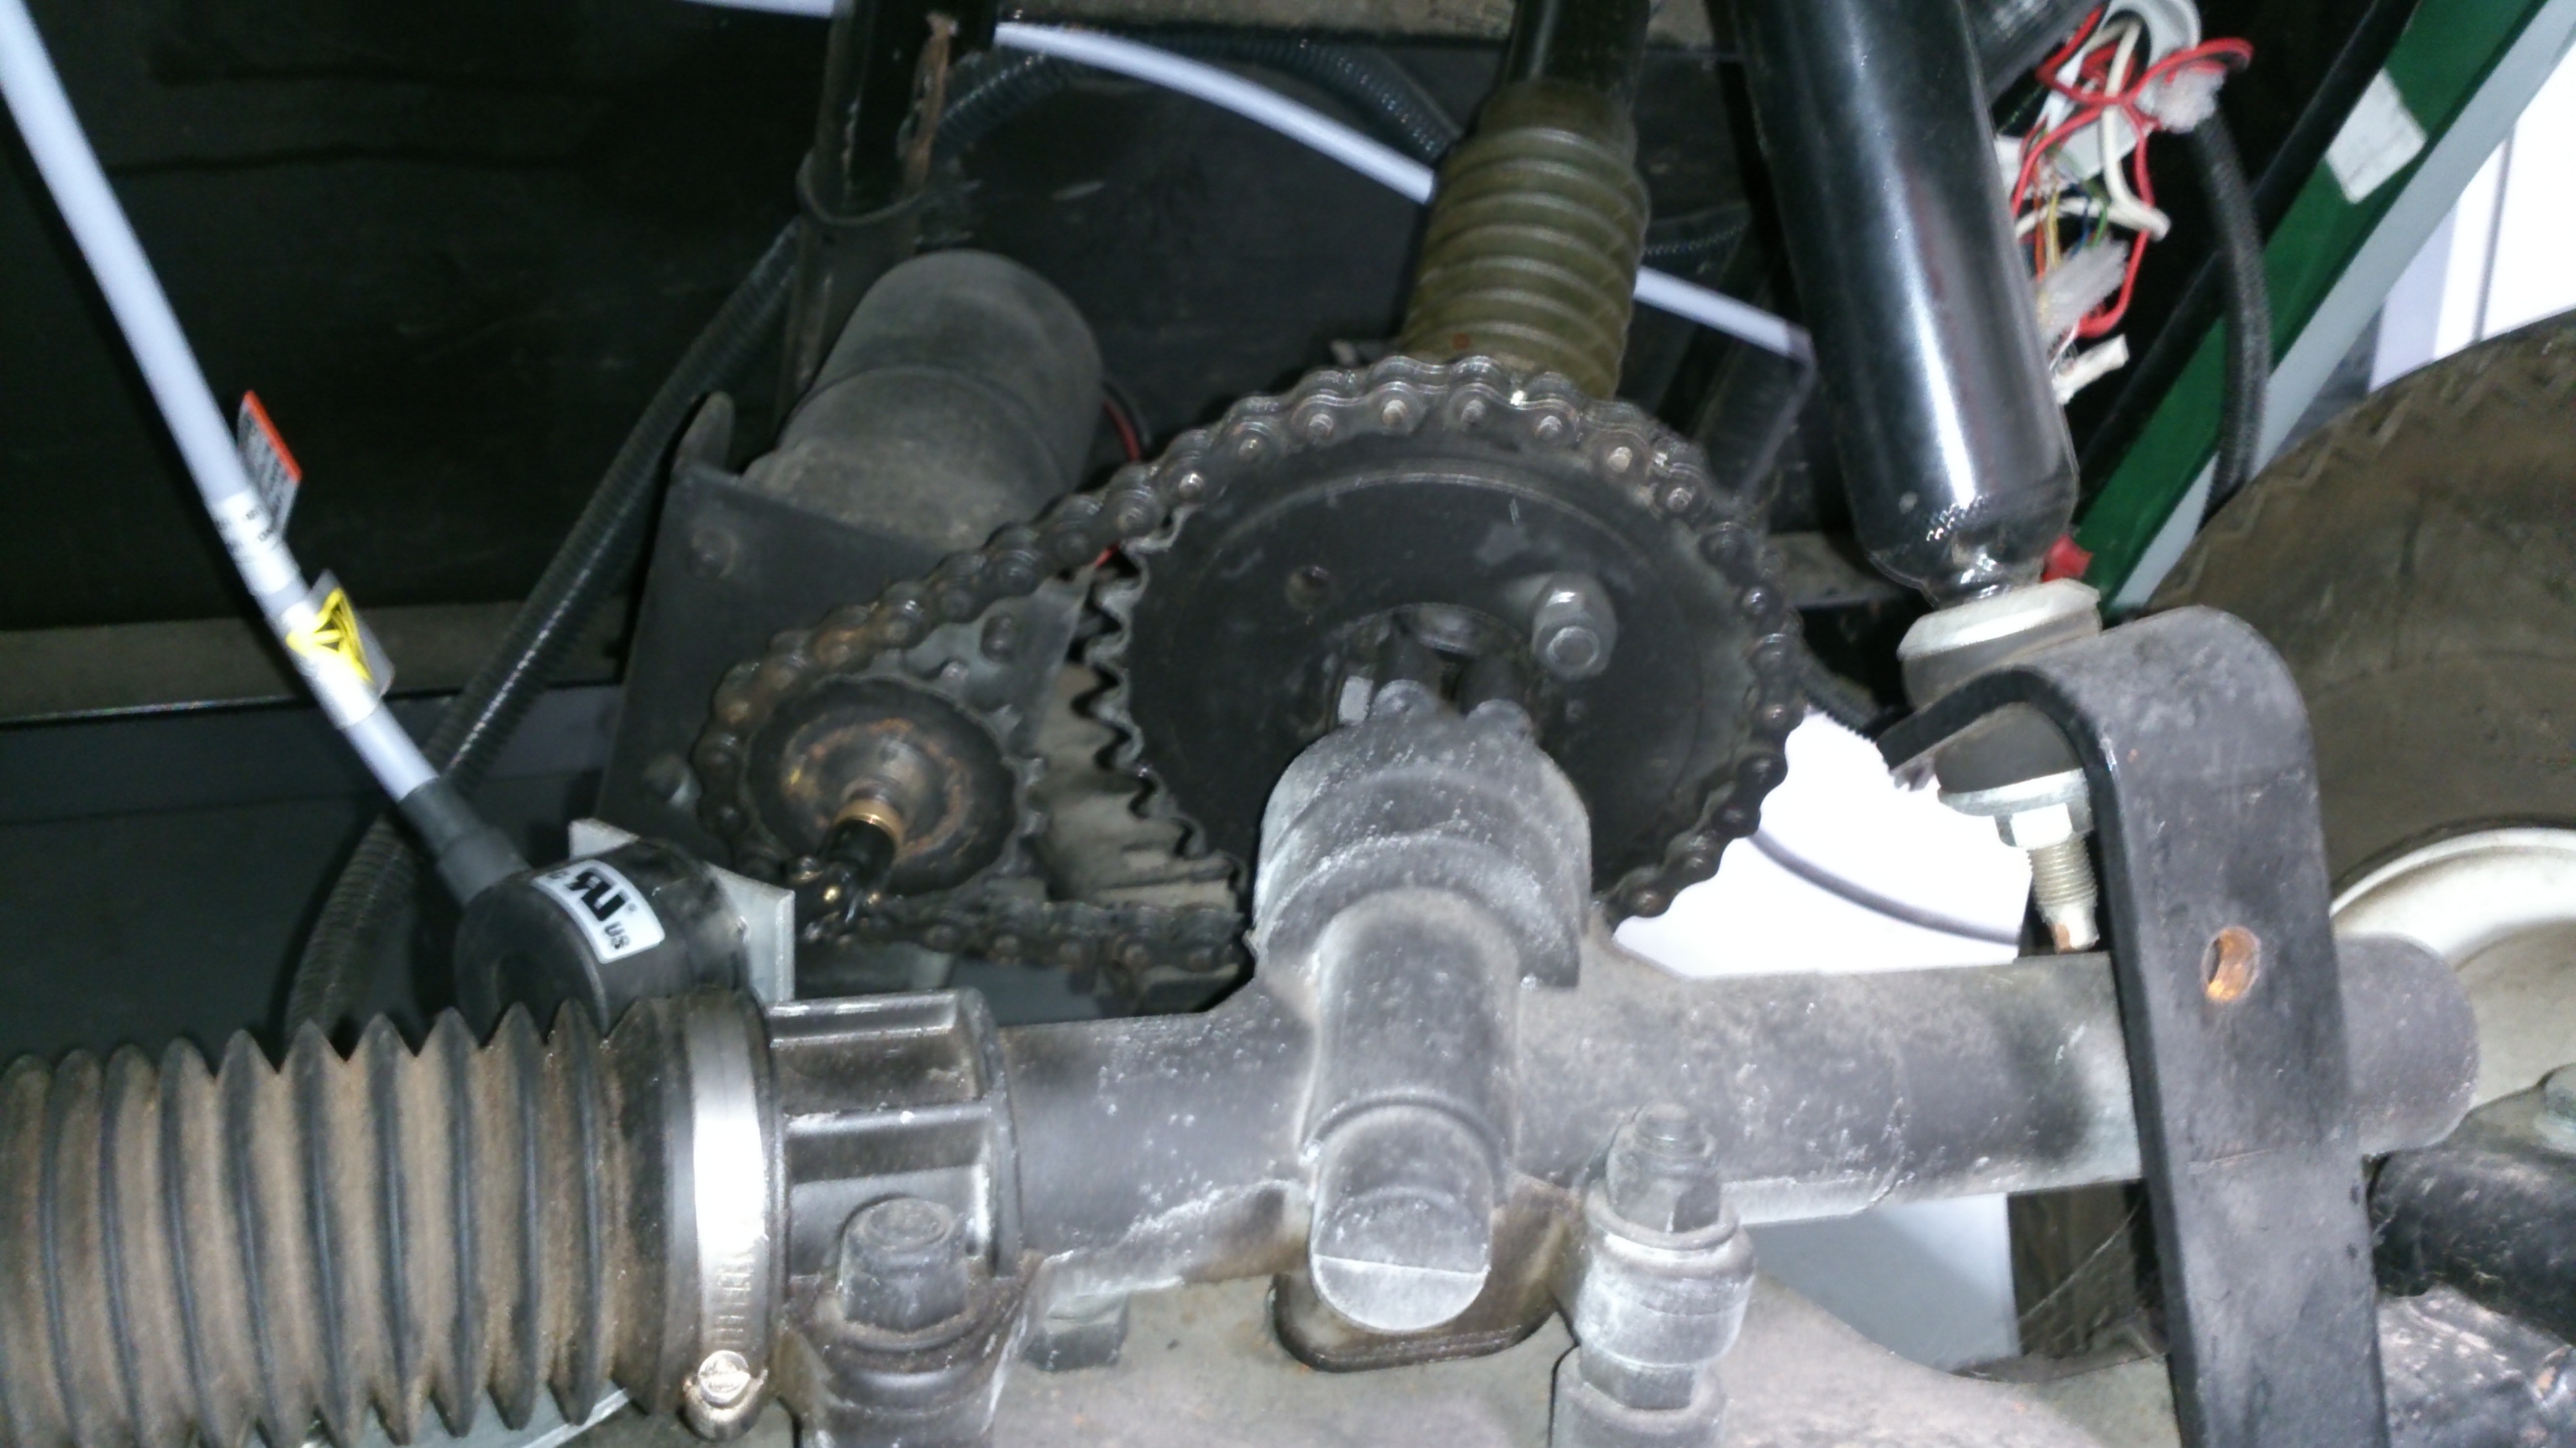
\includegraphics[width=\textwidth]{steering}
                \caption{Steering system.}\label{fig:cp00_steering}
        \end{subfigure}%        
        ~ %add desired spacing between images, e. g. ~, \quad, \qquad etc.
          %(or a blank line to force the subfigure onto a new line)
        \begin{subfigure}[b]{0.24\textwidth}
                \centering
                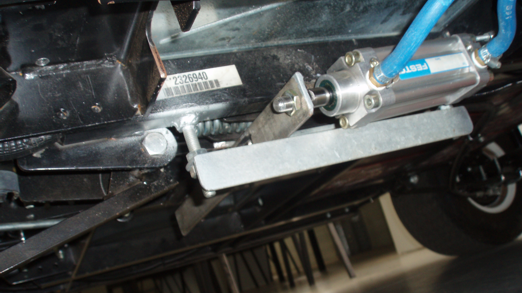
\includegraphics[width=\textwidth]{braking}
		\caption{Braking system.}\label{fig:cp00_brake}
        \end{subfigure}%
        ~ %add desired spacing between images, e. g. ~, \quad, \qquad etc.
          %(or a blank line to force the subfigure onto a new line)
        \begin{subfigure}[b]{0.24\textwidth}
                \centering
                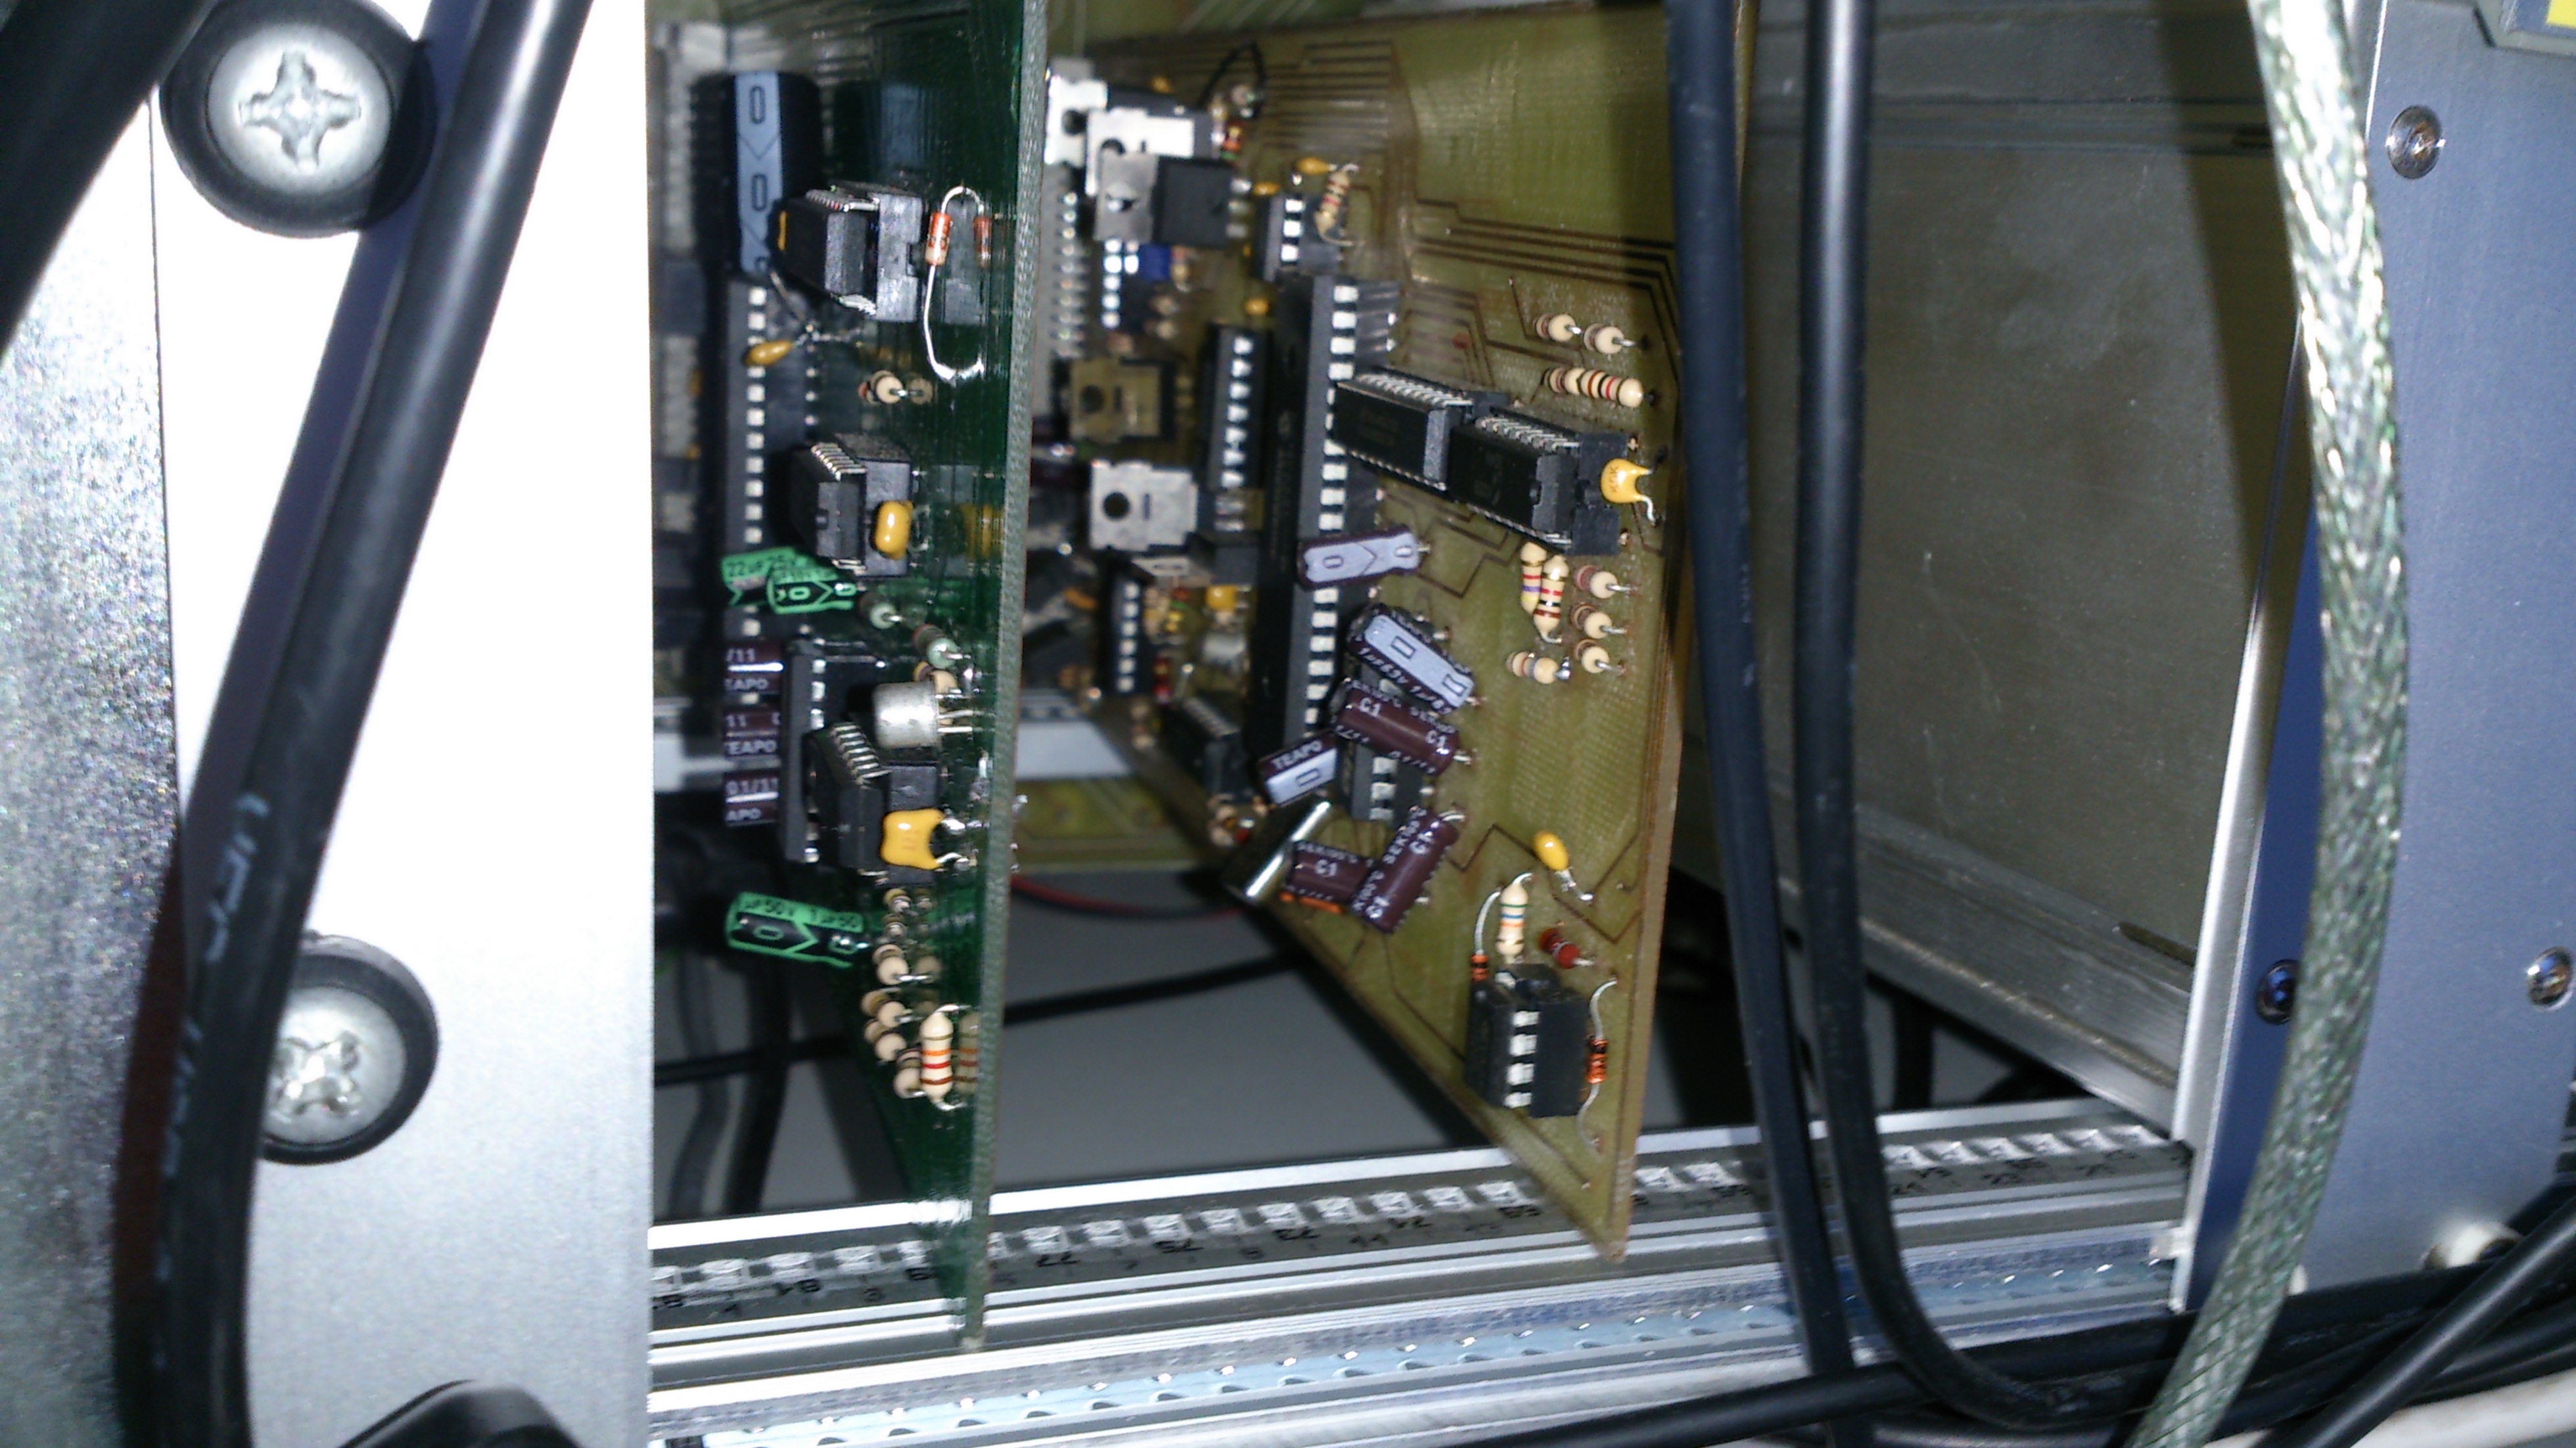
\includegraphics[width=\textwidth]{speed}
                \caption{Speed system.}\label{fig:cp00_speed}
        \end{subfigure}%
        ~
        \begin{subfigure}[b]{0.24\textwidth}
                \centering
                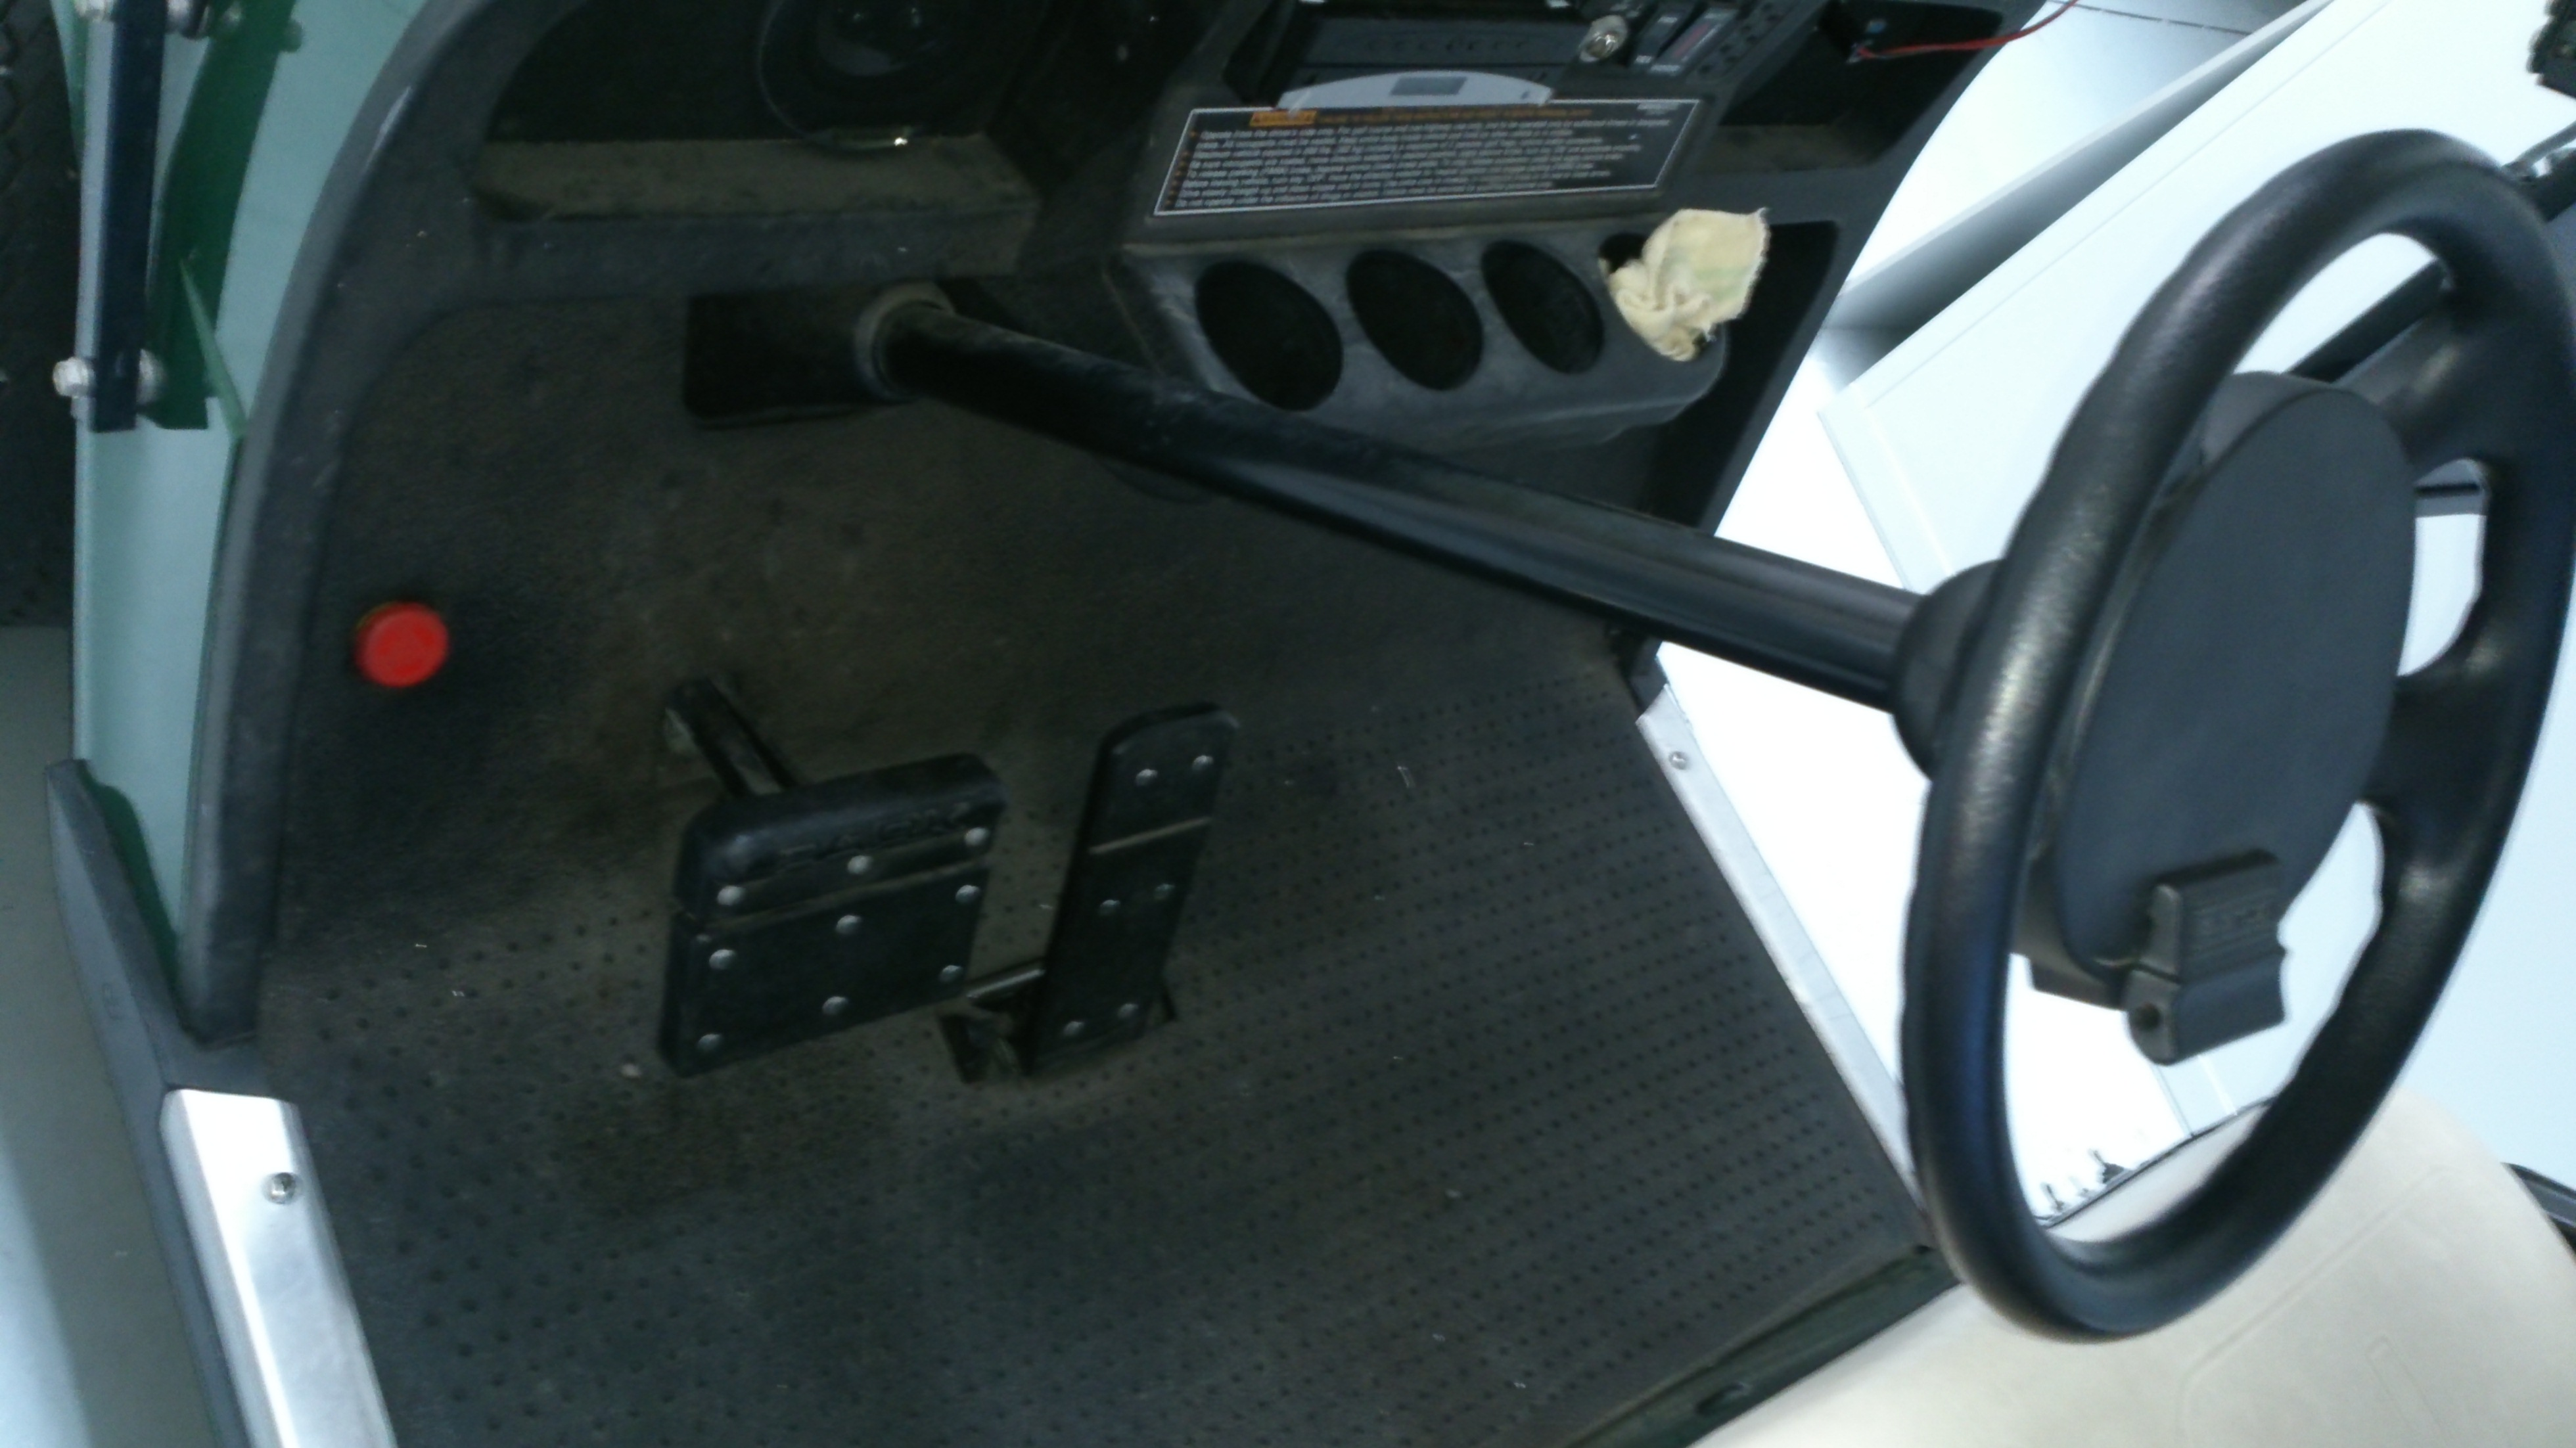
\includegraphics[width=\textwidth]{safety}
                \caption{Safety switch.}\label{fig:cp00_safety_switch}
        \end{subfigure}%
        \caption{Actuators installed on Verdino.}\label{fig:cp00_actuators}
\end{figure*}

\paragraph{Sensors}\label{ch:chapter00_03_00_00_02}

~\\~\\We distinguishing two sets of sensors. The first group is used in localization tasks:

\begin{itemize}
 \item \emph{Odometry}: This system measures the independent movement of the two rear wheels, which are attached to an optical encoder. This allows computing the position, orientation and speed of the prototype incrementally (See figure \ref{fig:cp00_odometry}).
 \item \emph{\acf{IMU}}: It is comprised by 9 sensors (3 accelerometers, 3 gyroscopes and 3 magnetometers), which are fused in real time in order to get the three-dimensional orientation of the vehicle. The model of the sensor is a \emph{Xsens Mti}\footnote{\url{http://www.xsens.com}} (See figure \ref{fig:cp00_imu}).
 \item \emph{\acf{DGPS}}: Allows positioning the vehicle with centimetric accuracy. It is composed by two different devices, the reference station, which is fixed in a known place, and the rover station, which is installed on the vehicle. The model used is a \emph{JAVAD GNSS Triumph-1}\footnote{\url{http://www.javad.com}}, which has an horizontal precision below 1\,cm and a vertical precision around 1.5\,cm using \ac{DGPS}, at a frequency of $5\,Hz$ (See figure \ref{fig:cp00_dgps}).
\end{itemize}

\begin{figure*}[h!]
        \centering
        \begin{subfigure}[b]{0.32\textwidth}
                \centering
                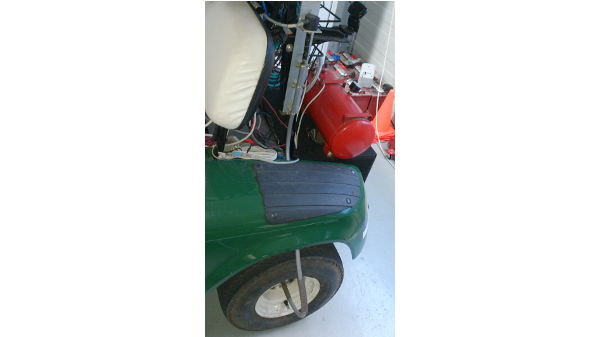
\includegraphics[width=\textwidth]{odometry}
                \caption{Odometry.}\label{fig:cp00_odometry}
        \end{subfigure}%        
        ~ %add desired spacing between images, e. g. ~, \quad, \qquad etc.
          %(or a blank line to force the subfigure onto a new line)
        \begin{subfigure}[b]{0.32\textwidth}
                \centering
                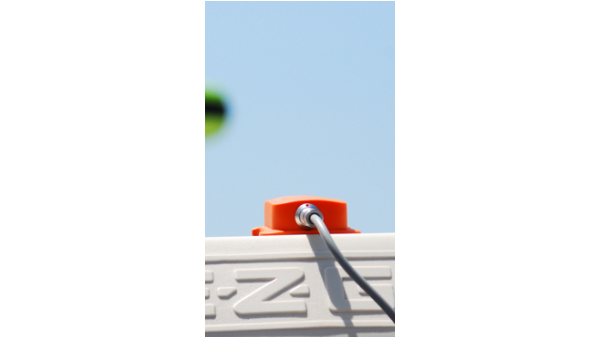
\includegraphics[width=\textwidth]{imu}
		\caption{\ac{IMU}.}\label{fig:cp00_imu}
        \end{subfigure}%
        ~ %add desired spacing between images, e. g. ~, \quad, \qquad etc.
          %(or a blank line to force the subfigure onto a new line)
        \begin{subfigure}[b]{0.32\textwidth}
                \centering
                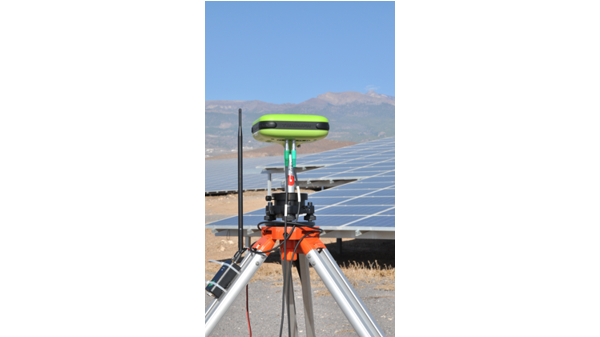
\includegraphics[width=\textwidth]{dgps}
                \caption{\ac{DGPS}.}\label{fig:cp00_dgps}
        \end{subfigure}%
        \caption{Localization sensors installed on Verdino.}\label{fig:cp00_localization_sensors}
\end{figure*}

The second group of sensors is oriented to the detection of the obstacles in the environment:

\begin{itemize}
 \item \emph{\acf{LIDAR}}: These are used also for localization purposes \citep{Perea2013mcl}. Each of those sensors is able to detect the objects in the way of the vehicle, at the plane in which the sensor is mounted. The advantages of these sensors are that they have a high speed and precision. However, they are just able to detect obstacles that crosses the plane defined by the sensor. Because of this, we have equipped the vehicle with 5 \acp{LIDAR}. Two of them are located at the same plane in the front corners of the vehicle, at a height of 50\,cm. Each of these covers an angle of 270\textdegree. Another is located in the front side of the vehicle, at a height of 20\,cm, slightly tilted upwards, in order to detect the small obstacles or non traversable areas. Another is in the top of the vehicle, also in the front side of the vehicle, tilted to the ground and covering the blind areas left by the other sensors. Finally, the last sensor is situated in the back side of the vehicle, and it is used for backwards maneuvers. The used sensors are of the model \emph{SICK LMS 100} and \emph{SICK LMS 111}\footnote{\url{http://www.sick.com}}, allowing a maximal detection distance of 20\,m, a precision of 10-35\,mm, a maximal angular resolution of 0.25\textdegree and a maximal rate of $50\,Hz$ (See figure \ref{fig:cp00_lidar}).
 \item \emph{IR cameras}: Infrared cameras are used to detect pedestrians or animals based on their temperature. We have a pair of them installed on a Pan-Tilt system attached to the top front side of the vehicle. The model used is a \emph{MobiR\textregistered~M3}\footnote{\url{http://www.guide-infrared.com}}, which is able to detect objects in the range $8\sim14\mu m$, at a resolution of $160 \times 120\,px$ (See figure \ref{fig:cp00_ir_cameras}).
 \item \emph{Visible cameras}: A set of three cameras is also installed in a pan-tilt structure. These are used for the detection and tracking of the objects, which is one of the goals of this thesis. Also, they are currently being used for the detection of the borders of the road \citep{arnay2009applying}. The model of the cameras is a \emph{GoPro\textregistered Hero 3 silver edition}\footnote{\url{http://gopro.com}}, with a $1920 \times 1080 \, px$ maximal video resolution and a 170\textdegree field of view at a maximal rate of 60\,fps (See figure \ref{fig:cp00_visible_cameras}).
\end{itemize}

\begin{figure*}[h!]
        \centering
        \begin{subfigure}[b]{0.32\textwidth}
                \centering
                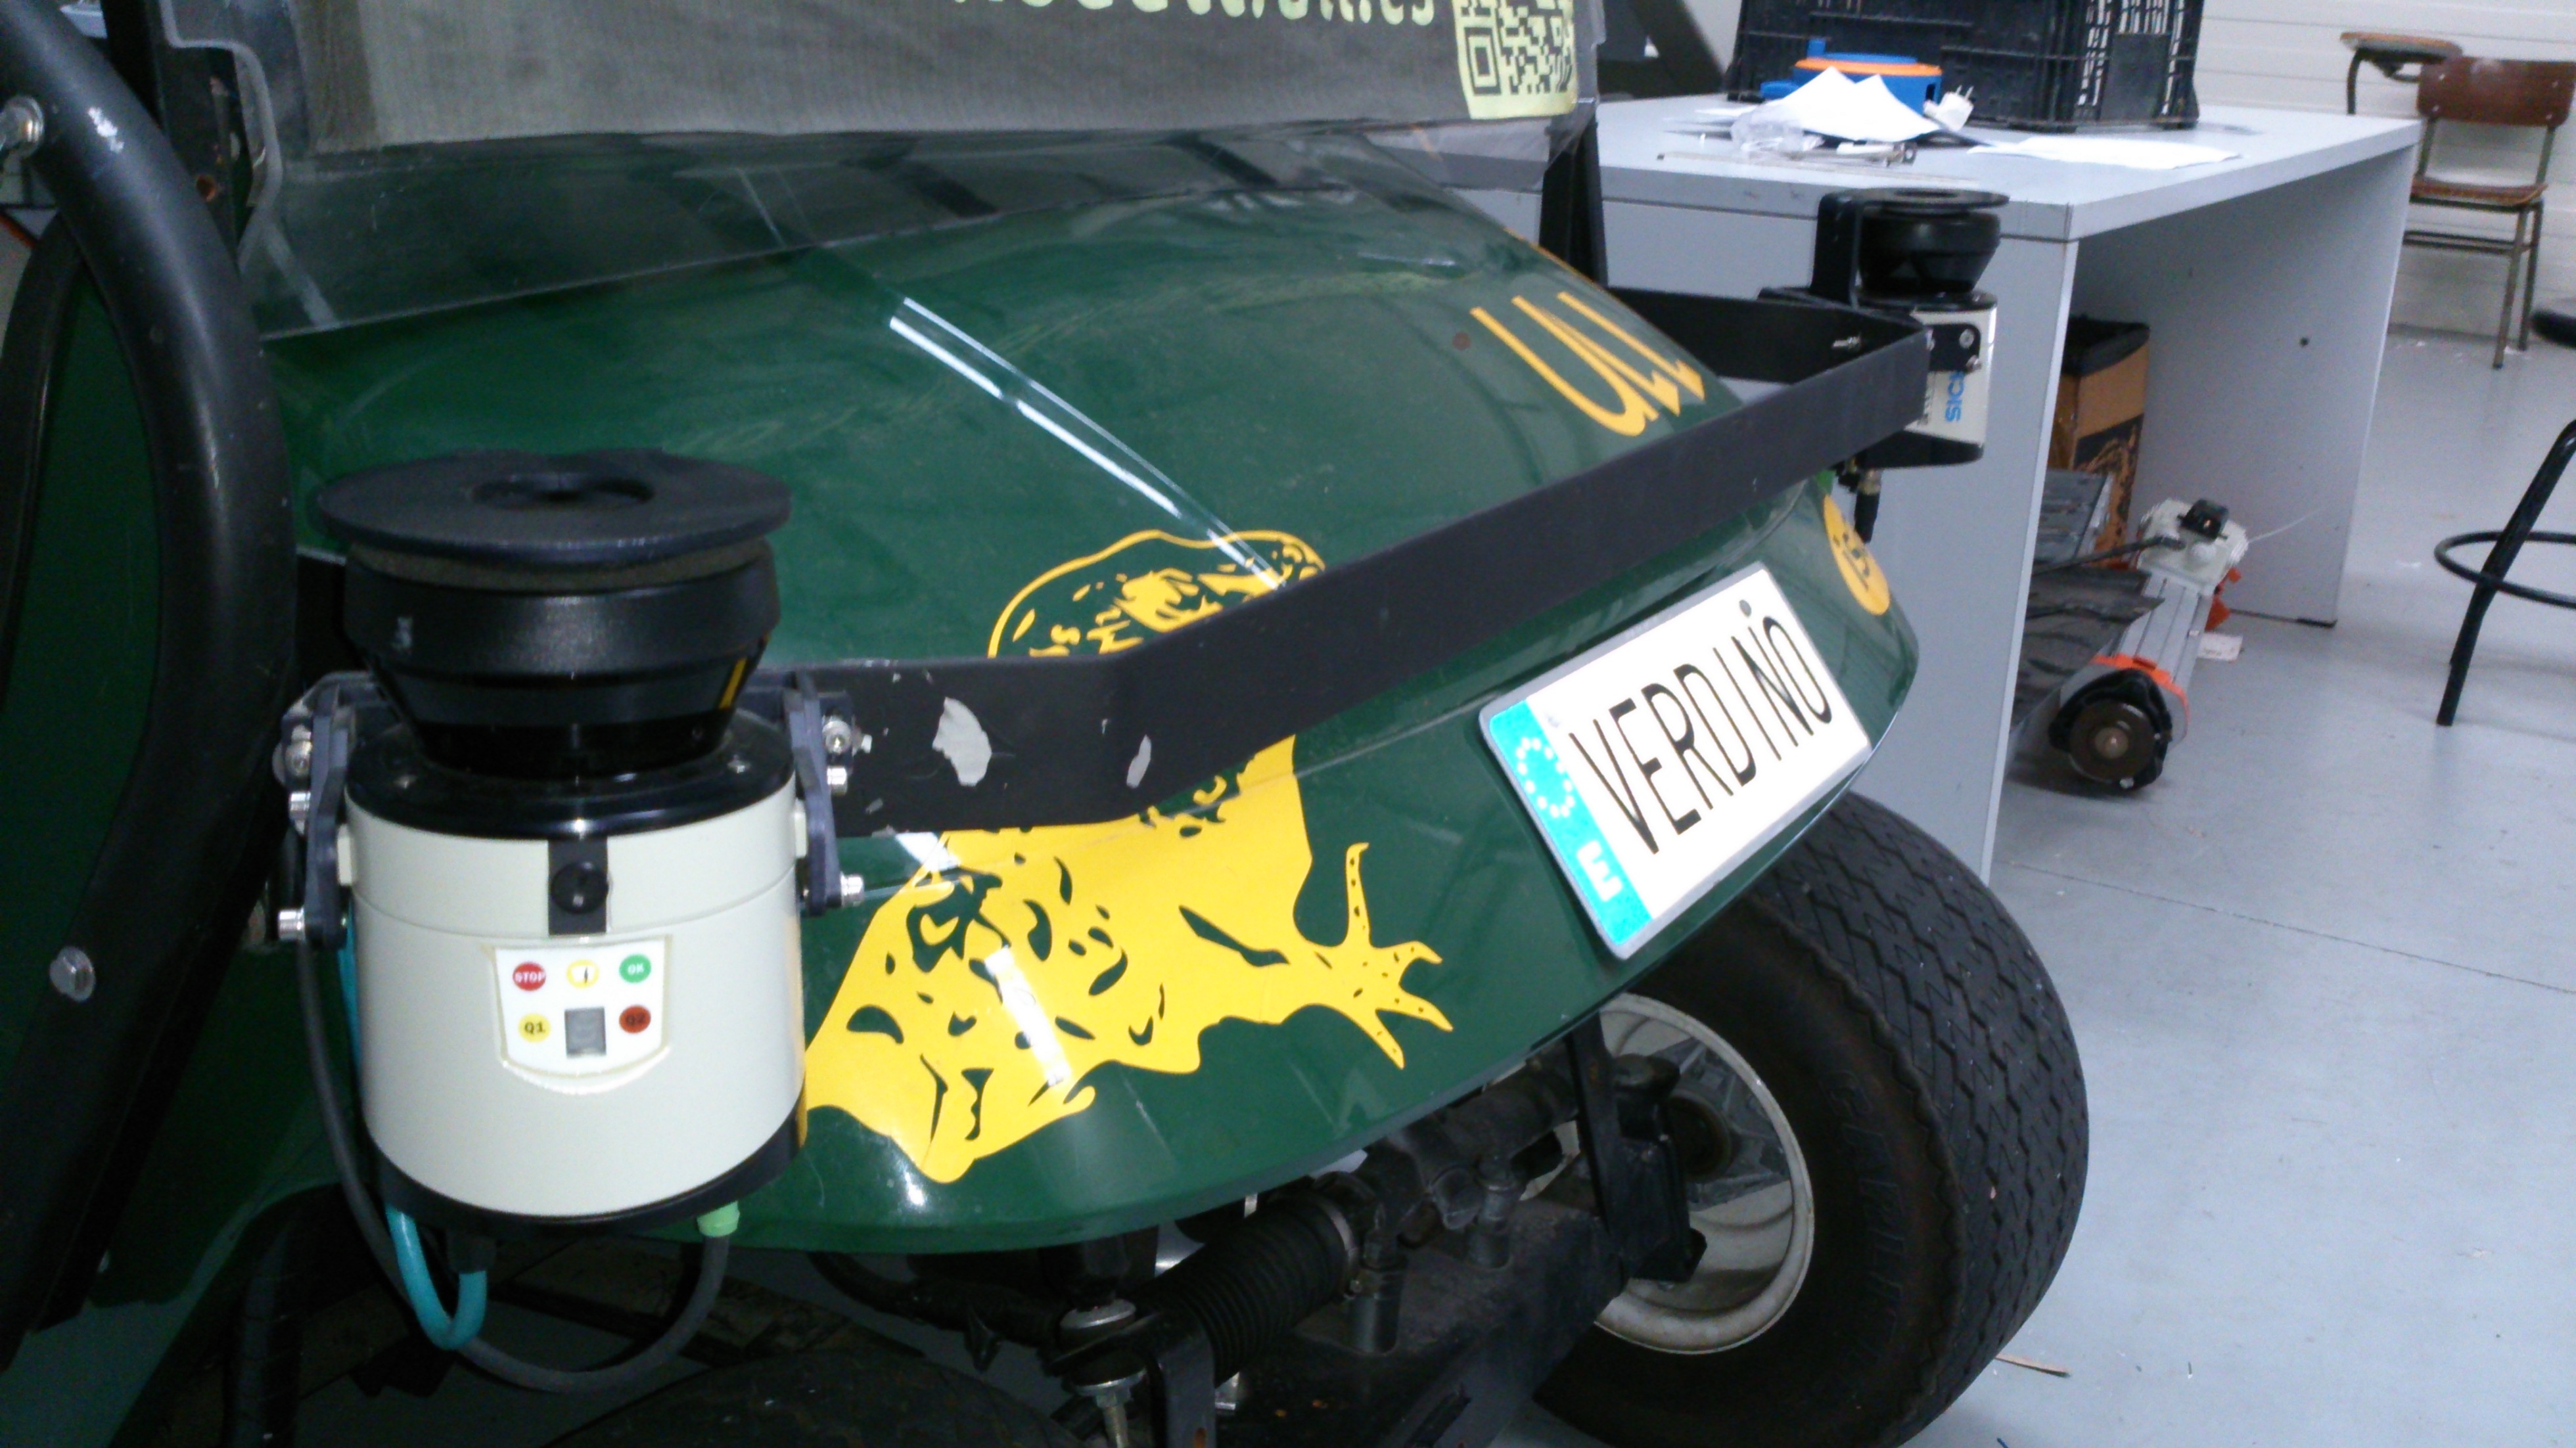
\includegraphics[width=\textwidth]{lidar}
                \caption{\ac{LIDAR}.}\label{fig:cp00_lidar}
        \end{subfigure}%        
        ~ %add desired spacing between images, e. g. ~, \quad, \qquad etc.
          %(or a blank line to force the subfigure onto a new line)
        \begin{subfigure}[b]{0.32\textwidth}
                \centering
                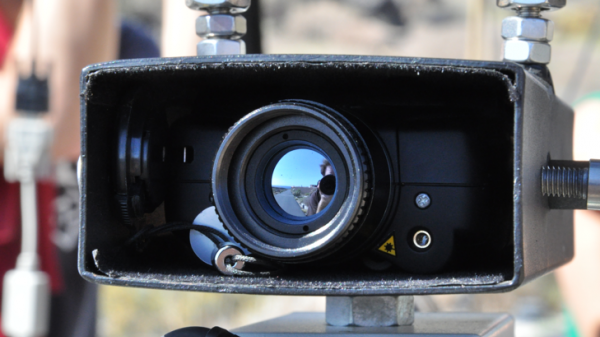
\includegraphics[width=\textwidth]{ircameras}
		\caption{IR Cameras.}\label{fig:cp00_ir_cameras}
        \end{subfigure}%
        ~ %add desired spacing between images, e. g. ~, \quad, \qquad etc.
          %(or a blank line to force the subfigure onto a new line)
        \begin{subfigure}[b]{0.32\textwidth}
                \centering
                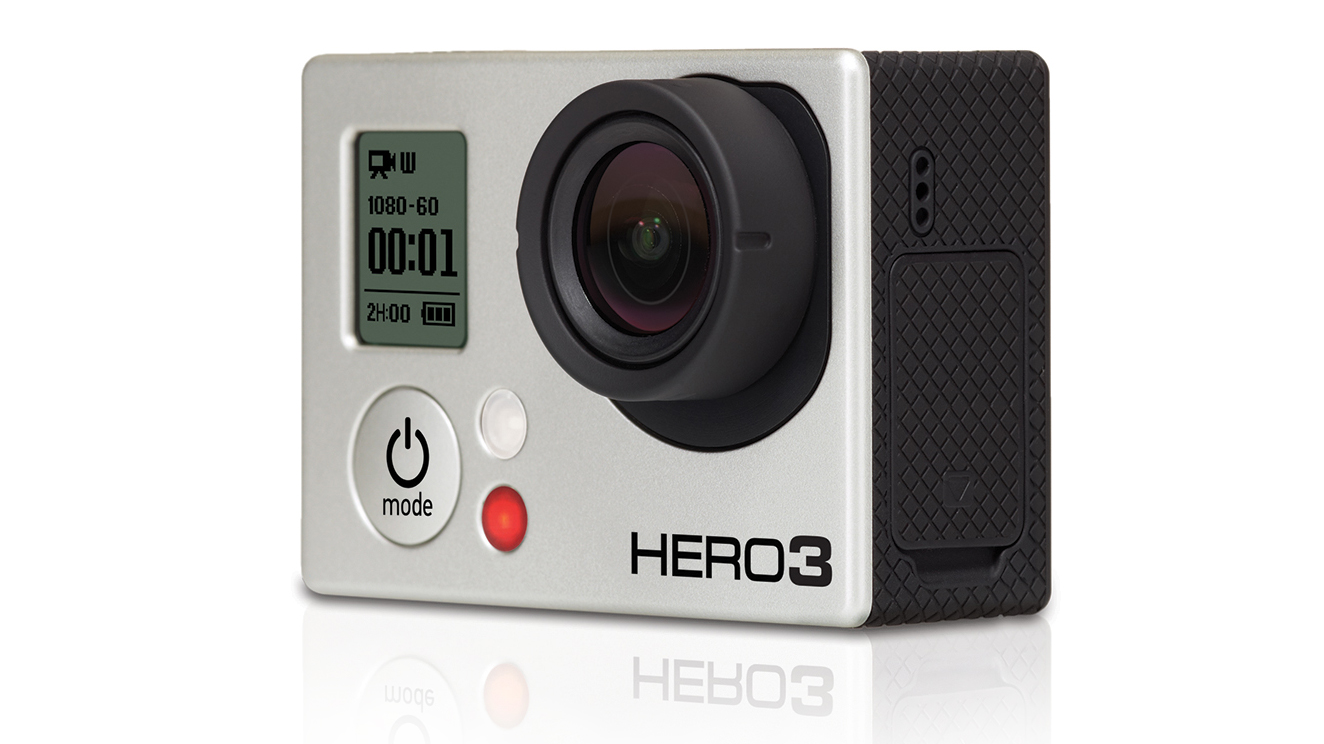
\includegraphics[width=\textwidth]{visiblecamera}
                \caption{Visible Cameras.}\label{fig:cp00_visible_cameras}
        \end{subfigure}%
        \caption{Obstacle detection sensors installed on Verdino.}\label{fig:cp00_detection_sensors}
\end{figure*}

\paragraph{Control}\label{ch:chapter00_03_00_00_03}

~\\~\\The vehicle is controlled, at high level, by an on board computer equipped with an \emph{i7-3770K} processor, 16\,Gb of \emph{RAM DDR-3} memory and a \emph{SSD} storage. At low level, a set of own developed electronic devices receive commands from the computer and transform them into the right signal, understandable by the actuators described before.

\section{Summary}\label{ch:chapter00_04}

In this chapter, we have done an initial description of the work presented in this thesis. Also, the pipeline of the final developed application is introduced. All this information will be explained in more detail in the following sections, including implementation details as well as some results, and a discussion of the advantages/disadvantages of the different methods.